\chpt{Experimental methodology} \label{ch:methodology}

\section{Organisation of the pedagogical experiment} \label{sec:organisation}

\subsection{Institutional context}

The pedagogical experiment was conducted at the Centre for Pre-University Training and Education (CDPO) of Kryvyi Rih State Pedagogical University (KDPU), Ukraine~\cite{KSPU}. CDPO offers preparatory courses for prospective university applicants preparing for the National Multi-Subject Test (NMT) -- Ukraine's standardised university entrance examination~\cite{Lokshyna2018302}. The Ukrainian History component of the NMT covers the entire school curriculum from ancient times to the present day, requiring comprehensive knowledge across all historical periods.

The course was delivered entirely via distance learning~\cite{Hlianenko2024, Zamkova2023299}, reflecting both the institutional adoption of online education since the COVID-19 pandemic and the ongoing security situation due to Russia's full-scale invasion of Ukraine, which began on February 24, 2022~\cite{Martynets202428, Vovchasta2024, Maslova2021}. The city of Kryvyi Rih, located in Dnipropetrovsk Oblast, experienced regular missile and drone attacks throughout the study period, directly affecting participants' ability to attend synchronous sessions~\cite{Zamkova2023299}.

The research was conducted within the framework of the scientific topic ``ICT-based learning environment of the university as a factor of professional development of the future specialist'' (state registration No.~0120U101116, dated 26.02.2020). The course was organised according to the approved syllabus (``Робоча навчальна програма'') and calendar-thematic plan (``Календарно-тематичний план''), both archived in the repository's \texttt{Lecture material/} directory. The instructional structure comprised 40 lectures, 40 seminars, and 7 modular controls delivered over approximately seven months, following the standard CDPO preparatory course format~\cite{KSPU}.

The experimental design was directly informed by the author's prior theoretical and methodological work. Two systematic reviews~\cite{KorniienkoSemerikov2024, Korniienko2025aredu} established the evidence base for gamification in history education and identified five implementation archetypes. The MRQS quality assessment~\cite{Korniienko2025mrqs} revealed pervasive methodological weaknesses in the field (83.8\% of studies carried high risk of bias), motivating the present study's emphasis on transparent reporting and ecological validity. The DigComp alignment analysis~\cite{Titova2025cte} provided the digital competence framework, while the international context review~\cite{Korniienko2025cte} situated the experiment within global educational technology trends. These findings collectively shaped the six design principles operationalised in the experiment (Section~\ref{sec:principle-implications}).

\subsection{The National Multi-Subject Test (NMT)}

The NMT replaced the earlier ZNO (External Independent Evaluation) system beginning in 2022, adapting Ukraine's university entrance assessment to wartime conditions~\cite{MON}. The NMT for Ukrainian History encompasses the complete school history curriculum and requires competencies in:

\begin{itemize}
\item \textbf{Chronological knowledge}: Sequencing events across all historical periods from ancient times to the present;
\item \textbf{Factual recall}: Identifying key figures, dates, treaties, and events;
\item \textbf{Source analysis}: Interpreting primary sources including texts, maps, images, and statistical data;
\item \textbf{Cause and effect}: Explaining causal relationships between historical events and processes;
\item \textbf{Comparative analysis}: Identifying similarities and differences across historical periods and regions.
\end{itemize}

The test format includes multiple-choice questions, matching/correspondence tasks, chronological sequencing, and open-ended items~\cite{Lokshyna2018302}. Table~\ref{tab:nmt-format} summarises the NMT question types and their correspondence to the gamification elements used in this study.

\begin{table}[htbp]
\centering
\caption{NMT question types and corresponding gamification elements}
\label{tab:nmt-format}
\small
\begin{tabular}{p{3.5cm}p{4cm}p{5.5cm}}
\hline
\textbf{NMT question type} & \textbf{Cognitive demand} & \textbf{Gamification correspondence} \\
\hline
Multiple choice & Recognition, factual recall & Google Forms quiz blocks \\
Matching/correspondence & Association, categorisation & HistoryLikeGame drag-and-drop \\
Chronological sequencing & Temporal reasoning & HistoryLikeGame drag-and-drop \\
Source analysis & Interpretation, evaluation & Seminar source-based questions \\
Open-ended & Recall, synthesis & HistoryLikeGame text input \\
\hline
\end{tabular}
\end{table}

The NMT competencies map systematically to Bloom's revised taxonomy~\cite{Clark2016}: factual recall and chronological knowledge correspond to \emph{remember} and \emph{understand}; source analysis engages \emph{analyse} and \emph{evaluate}; cause-and-effect and comparative reasoning require \emph{apply} and \emph{evaluate}. This cognitive progression informed the scaffolding strategy for both Google Forms seminars and the HistoryLikeGame platform, where quiz types were selected to exercise specific cognitive levels (Section~\ref{sec:principle-grounding}).

The NMT's digital format -- administered entirely via computer -- directly engages DigComp Area~1 (Information and data literacy) through source evaluation and Area~5 (Problem solving) through digital test navigation~\cite{Vuorikari2016, Cosgrove2025}. The gamified platform thus served a dual purpose: NMT content preparation and implicit digital competence development (Section~\ref{sec:digcomp}).

The 2025 NMT was scheduled for May 14, 2025, providing the external deadline that shaped the course timeline and influenced student engagement patterns~\cite{Vuorikari2016}. The proximity of this deadline may have contributed to the observed variation in participation in later seminars (Section~\ref{ch:results}).

Figure~\ref{fig:visual-sources} illustrates the visual source analysis component of the course materials, showing the type of historical portrait identification exercises that correspond to the NMT source analysis question format.

\begin{figure}[htbp]
\centering

\includegraphics[width=0.7\textwidth]{posibnyk_4_visual_sources.jpg}
\caption{Course material: visual source identification exercise featuring historical portraits of key Ukrainian figures (Mazepa, Hrushevskyi, Petliura, Stalin) with associated artifacts}
\label{fig:visual-sources}
\end{figure}

\subsection{Participants}

Twenty-three students enrolled in the NMT preparatory course for Ukrainian History during the study period. Enrolment was open and occurred on a rolling basis, with the complete enrollment timeline reconstructed from the Viber chat log join events (Table~\ref{tab:enrollment-detail}).

\begin{table}[htbp]
\centering
\caption{Detailed enrollment timeline from chat log analysis}
\label{tab:enrollment-detail}
\small
\begin{tabular}{clcc}
\hline
\textbf{No.} & \textbf{Date} & \textbf{Phase} & \textbf{Cumulative} \\
\hline
1 & 2024-10-01 & Phase 1 & 1 \\
2 & 2024-10-04 & Phase 1 & 2 \\
3--6 & 2024-10-06--08 & Phase 1 & 6 \\
7--9 & 2024-10-09--11 & Phase 1 & 9 \\
10 & 2024-10-16 & Phase 1 & 10 \\
11 & 2024-10-25 & Phase 1 & 11 \\
12--17 & 2024-11-01--13 & Phase 2 & 17 \\
18--19 & 2025-01-22--27 & Phase 3 & 19 \\
20--21 & 2025-02-13--25 & Phase 3 & 21 \\
22 & 2025-03-03 & Phase 3 & 22 \\
23 & 2025-04-11 & Phase 3 & 23 \\
\hline
\end{tabular}
\end{table}

The three enrollment phases -- rapid initial formation (October, N=11), gradual expansion (November, N=6), and late enrollment (January--April, N=6) -- reflect distinct student motivations, from early commitment through word-of-mouth recruitment to last-minute decisions to seek structured preparation. The enrollment timeline is detailed in Table~\ref{tab:enrollment-detail} and analysed further in Section~\ref{sec:baseline}.

The rolling enrollment pattern is typical for CDPO preparatory courses and reflects the open-access nature of the programme. Participants were predominantly secondary school graduates or final-year students preparing for the 2025 NMT examination~\cite{MON}. Demographic data were limited by the course format; individual identification was possible through the names provided in Google Forms responses and the Viber chat group.

The cumulative enrollment curve is visualised in Figure~\ref{fig:enrollment} (Section~\ref{sec:baseline}), showing the step-function pattern characteristic of open-access preparatory courses.

The sample size of N=23 warrants methodological contextualisation. The systematic review (Section~\ref{sec:evidence-base}) found that the median sample size across gamification studies in history education was N=33.5, with substantial variation (range: 8--1,031). Several methodologically rigorous studies operated with comparable or smaller samples~\cite{Yin2018, CohenManionMorrison2018}. The present study prioritises ecological validity -- the experiment took place within an authentic educational programme, not an artificial laboratory setting~\cite{WangHannafin2005, AndersonShattuck2012}. This design-based research approach~\cite{Bakker2018} treats the naturalistic setting as a strength rather than a limitation, enabling observation of genuine pedagogical dynamics including the wartime disruptions that constitute an essential contextual variable. Furthermore, as~\cite{WangHannafin2005} argue, DBR studies typically work with intact groups in real settings, where the research question concerns not ``does it work?'' but ``how does it work, for whom, and under what conditions?'' --- questions that require rich contextual data rather than large-N statistical power. The individual trajectory analysis (Section~\ref{sec:formative}) demonstrates the analytical possibilities afforded by detailed longitudinal tracking of each participant across 36 assessment points.

Ethical considerations: As the study employed an ex post facto design~\cite{creswell, ary} analysing data collected during regular educational activities (not designed as research), no separate informed consent for research participation was required under the Law of Ukraine ``On Education''~\cite{ZakonOsvita2017}. All data were anonymised using the purpose-built \texttt{anonymize\_names.py} script, which replaced participant names with consistent pseudonyms across all data files. Student names were used only for internal trajectory analysis and replaced with initials or codes in all publications and presentations. The research adhered to the ethical principles outlined by~\cite{CohenManionMorrison2018} for educational research involving routine pedagogical data. All original data sources --- Viber chat log exports, Google Forms response files (XLSX/CSV), Zoom recordings, and HistoryLikeGame source code --- are preserved in the research repository, enabling full reproducibility of the analysis pipeline described in Section~\ref{sec:data-analysis}.

\subsection{Research design}

\subsubsection{Design justification}

The study employed an ex post facto single-group repeated-measures design~\cite{creswell, ary}, situated within the design-based research (DBR) paradigm~\cite{WangHannafin2005, AndersonShattuck2012, Bakker2018}. This methodological choice was determined by three contextual constraints:

\begin{enumerate}
\item \textbf{Ethical and institutional constraints.} The educational context did not permit random assignment to treatment and control groups, as all enrolled students were entitled to the same educational services~\cite{Sanina2020}. Creating a ``no-gamification'' control group would have been ethically problematic in a high-stakes NMT preparation context~\cite{CampbellStanley1963, ShadishCookCampbell2002};
\item \textbf{Ecological validity priority.} The primary interest was in documenting the implementation process and tracking performance over time within a real educational setting, consistent with the DBR emphasis on naturalistic intervention~\cite{Reeves20033, WangHannafin2005}. The systematic review identified that only 31.1\% of gamification studies in history education include control groups (Section~\ref{sec:evidence-base}), and the MRQS analysis revealed that 83.8\% carry high risk of bias (Section~\ref{sec:qa-results}). The present study addresses this limitation through transparent reporting rather than artificial experimental control;
\item \textbf{Wartime context.} The ongoing armed conflict introduced variables (power outages, missile alerts, internet disruptions, forced displacement) that could not be controlled experimentally but constituted important contextual and moderating factors~\cite{Martynets202428, UNESCO2023, Burde2017, Kirk2007}.
\end{enumerate}

This design aligns with the acknowledged need in the field (Section~\ref{sec:mrqs}) for studies that prioritise ecological validity and comprehensive documentation over artificial experimental control~\cite{Korniienko2025mrqs, Hamari2014, DichevDicheva2017}. As~\cite{AndersonShattuck2012} note, design-based research is particularly appropriate when the intervention is deeply embedded in its context and cannot be meaningfully separated from it. The iterative nature of DBR --- where findings from early implementation cycles inform subsequent design refinements --- is reflected in the phased introduction of gamification elements: the initial HistoryLikeGame deployment (December~1, 2024) was followed by the later addition of Wordwall (March~27, 2025), representing a second design iteration informed by observed engagement patterns~\cite{Bakker2018}.

The methodological position adopted here follows~\citeauthor{Yin2018}'s~\cite{Yin2018} argument that single-case designs are appropriate when the case is ``revelatory'' --- representing a situation previously inaccessible to research. The intersection of gamified history education, wartime distance learning, and NMT preparation constitutes such a revelatory case, as no prior study has examined gamification under comparable conditions of sustained armed conflict~\cite{Burde2017, Kirk2007}.

\subsubsection{Variable operationalisation}

Table~\ref{tab:variable-operationalization} presents the systematic operationalisation of all research variables, mapping each to its measurement instrument and the thesis section where it is analysed. Following \citeauthor{CohenManionMorrison2018}, each theoretical construct is linked to an observable, measurable indicator. The distinction between moderating and confounding variables is critical: enrollment timing and topic difficulty can be accounted for analytically, whereas self-selection bias (voluntary enrollment) remains an acknowledged limitation.

\begin{table}[htbp]
\centering
\caption{Operationalisation of research variables}
\label{tab:variable-operationalization}
\small
\begin{tabular}{p{1.8cm}p{2.5cm}p{3.2cm}p{2.2cm}p{1.8cm}}
\hline
\textbf{Type} & \textbf{Variable} & \textbf{Operationalisation} & \textbf{Measurement} & \textbf{Section} \\
\hline
Independent (treatment) & Gamification intervention & HistoryLikeGame platform, introduced Dec~1, 2024 & Binary pre/post & \ref{sec:gamification-design} \\
Independent (context) & Wartime conditions & Power/internet disruptions & Absence categories & \ref{sec:wartime-context} \\
Dependent (primary) & Academic performance & Quiz scores (\% of max) & Mean, SD & \ref{sec:formative} \\
Dependent (secondary) & Engagement & Participation rate per seminar & N per session & \ref{sec:formative} \\
Dependent (secondary) & Attendance persistence & Absence frequency and reasons & Categorical count & \ref{sec:attendance} \\
Moderating & Enrollment timing & Phase 1/2/3 join date & Days since start & Tab~\ref{tab:enrollment-detail} \\
Moderating & Topic difficulty & NMT curriculum section 1--4 & Lecture grouping & \ref{sec:discussion} \\
Confounding & Self-selection & Voluntary enrollment & Not controlled & Limitation \\
\hline
\end{tabular}
\end{table}

\subsubsection{Experimental logic model}

Figure~\ref{fig:logic-model} presents the logic model connecting the theoretical foundations established in Chapter~1 to the intervention components described in this chapter and the measured outcomes analysed in Chapter~3. This model operationalises the design space framework from Section~\ref{sec:principle-implications}, showing how each theoretical construct informed specific intervention decisions.

\begin{figure}[htbp]
\centering
\resizebox{\textwidth}{!}{%
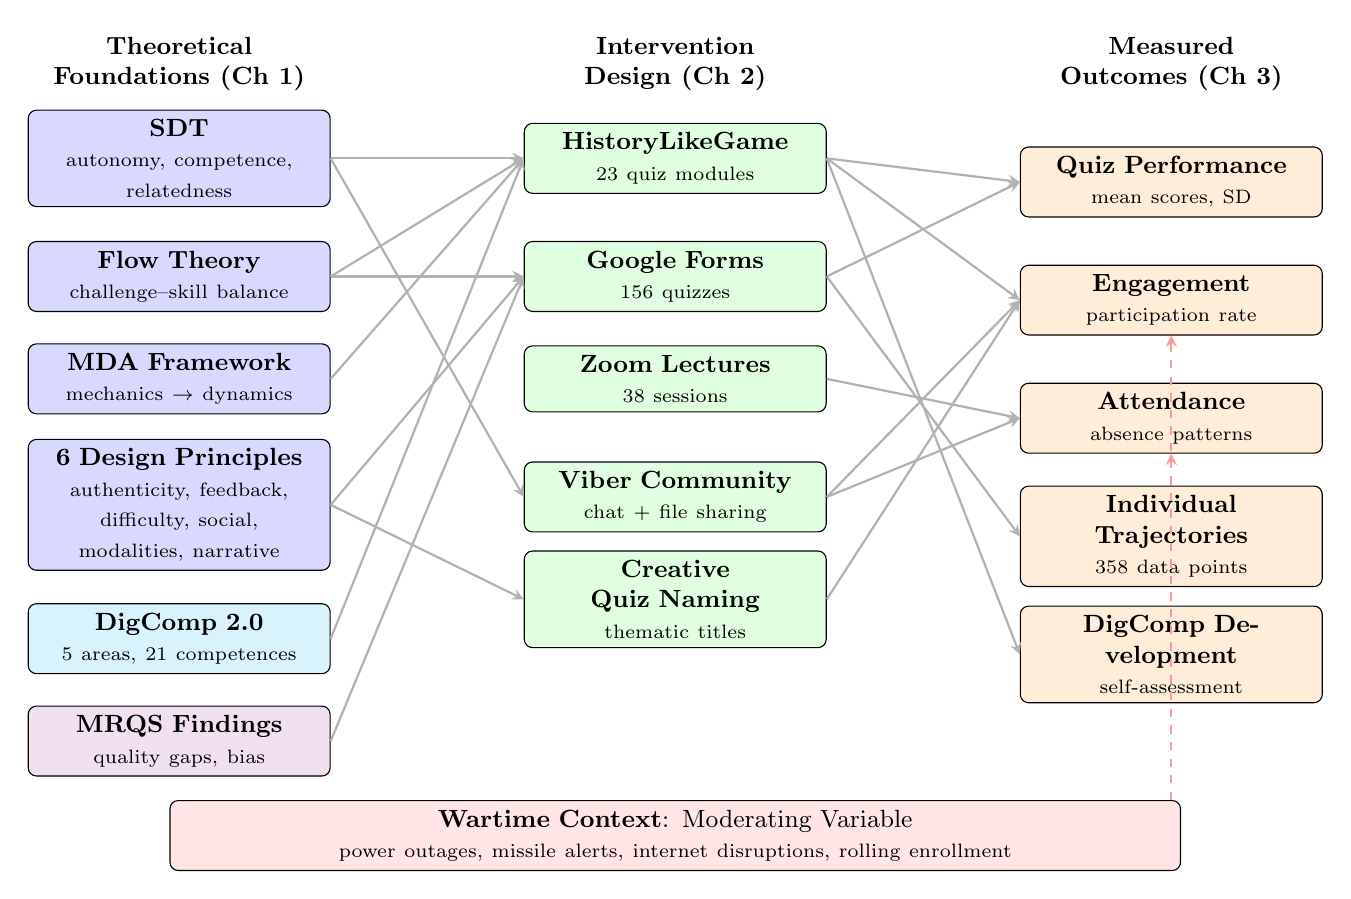
\begin{tikzpicture}[
  node distance=0.4cm,
  theorybox/.style={rectangle, draw, rounded corners=3pt, fill=blue!15,
    text width=3.6cm, minimum height=0.7cm, align=center, font=\small},
  intbox/.style={rectangle, draw, rounded corners=3pt, fill=green!12,
    text width=3.6cm, minimum height=0.7cm, align=center, font=\small},
  outbox/.style={rectangle, draw, rounded corners=3pt, fill=orange!15,
    text width=3.6cm, minimum height=0.7cm, align=center, font=\small},
  colhead/.style={font=\bfseries\small, align=center},
  arr/.style={->, >=stealth, thick, gray!60},
  warbar/.style={rectangle, draw, rounded corners=3pt, fill=red!10,
    minimum height=0.7cm, align=center, font=\small}
]

% Column headers
\node[colhead] (h1) at (0, 0) {Theoretical\\Foundations (Ch~1)};
\node[colhead] (h2) at (6.3, 0) {Intervention\\Design (Ch~2)};
\node[colhead] (h3) at (12.6, 0) {Measured\\Outcomes (Ch~3)};

% Column 1: Theory
\node[theorybox] (sdt) at (0, -1.2) {\textbf{SDT}\\{\scriptsize autonomy, competence,}\\{\scriptsize relatedness}};
\node[theorybox] (flow) at (0, -2.7) {\textbf{Flow Theory}\\{\scriptsize challenge--skill balance}};
\node[theorybox] (mda) at (0, -4.0) {\textbf{MDA Framework}\\{\scriptsize mechanics $\to$ dynamics}};
\node[theorybox] (principles) at (0, -5.6) {\textbf{6 Design Principles}\\{\scriptsize authenticity, feedback,}\\{\scriptsize difficulty, social,}\\{\scriptsize modalities, narrative}};
\node[theorybox, fill=cyan!15] (digcomp) at (0, -7.3) {\textbf{DigComp 2.0}\\{\scriptsize 5 areas, 21 competences}};
\node[theorybox, fill=violet!12] (mrqs) at (0, -8.6) {\textbf{MRQS Findings}\\{\scriptsize quality gaps, bias}};

% Column 2: Intervention
\node[intbox] (hlg) at (6.3, -1.2) {\textbf{HistoryLikeGame}\\{\scriptsize 23 quiz modules}};
\node[intbox] (gforms) at (6.3, -2.7) {\textbf{Google Forms}\\{\scriptsize 156 quizzes}};
\node[intbox] (zoom) at (6.3, -4.0) {\textbf{Zoom Lectures}\\{\scriptsize 38 sessions}};
\node[intbox] (viber) at (6.3, -5.5) {\textbf{Viber Community}\\{\scriptsize chat + file sharing}};
\node[intbox] (naming) at (6.3, -6.8) {\textbf{Creative Quiz Naming}\\{\scriptsize thematic titles}};

% Column 3: Outcomes
\node[outbox] (perf) at (12.6, -1.5) {\textbf{Quiz Performance}\\{\scriptsize mean scores, SD}};
\node[outbox] (engage) at (12.6, -3.0) {\textbf{Engagement}\\{\scriptsize participation rate}};
\node[outbox] (attend) at (12.6, -4.5) {\textbf{Attendance}\\{\scriptsize absence patterns}};
\node[outbox] (traj) at (12.6, -6.0) {\textbf{Individual Trajectories}\\{\scriptsize 358 data points}};
\node[outbox] (dcomp) at (12.6, -7.5) {\textbf{DigComp Development}\\{\scriptsize self-assessment}};

% Arrows: Theory → Intervention
\draw[arr] (sdt.east) -- (hlg.west);
\draw[arr] (sdt.east) -- (viber.west);
\draw[arr] (flow.east) -- (hlg.west);
\draw[arr] (flow.east) -- (gforms.west);
\draw[arr] (mda.east) -- (hlg.west);
\draw[arr] (principles.east) -- (gforms.west);
\draw[arr] (principles.east) -- (naming.west);
\draw[arr] (digcomp.east) -- (hlg.west);
\draw[arr] (mrqs.east) -- (gforms.west);

% Arrows: Intervention → Outcomes
\draw[arr] (hlg.east) -- (perf.west);
\draw[arr] (hlg.east) -- (engage.west);
\draw[arr] (gforms.east) -- (perf.west);
\draw[arr] (gforms.east) -- (traj.west);
\draw[arr] (zoom.east) -- (attend.west);
\draw[arr] (viber.east) -- (attend.west);
\draw[arr] (viber.east) -- (engage.west);
\draw[arr] (naming.east) -- (engage.west);
\draw[arr] (hlg.east) -- (dcomp.west);

% Bottom bar: Wartime context (moderating variable)
\node[warbar, text width=12.6cm] (war) at (6.3, -9.8) {\textbf{Wartime Context}: Moderating Variable\\{\scriptsize power outages, missile alerts, internet disruptions, rolling enrollment}};

% Dashed arrows from wartime to affected outcomes
\draw[->, >=stealth, thick, red!40, dashed] (war.north -| attend.south) -- (attend.south);
\draw[->, >=stealth, thick, red!40, dashed] (war.north -| engage.south) -- (engage.south);

\end{tikzpicture}
%
}
\caption{Experimental logic model: theoretical foundations (Chapter~1) $\to$ intervention design (Chapter~2) $\to$ measured outcomes (Chapter~3), with wartime context as moderating variable}
\label{fig:logic-model}
\end{figure}

The logic model follows the programme theory approach~\cite{FunnellRogers2011}, making explicit the causal assumptions underlying the intervention. Each arrow represents a theoretically motivated design decision: SDT-informed autonomy is operationalised through voluntary game exploration; Flow-informed challenge--skill balance is implemented through progressive quiz difficulty; and the six design principles from Section~\ref{sec:design-principles} map directly to specific course components.

\subsubsection{Threats to validity}

Following~\cite{ShadishCookCampbell2002}, the key threats to validity are acknowledged:

\textbf{Internal validity.} Six threats are identified, following~\cite{CampbellStanley1963}:

\begin{enumerate}
\item \emph{History effects}: the wartime context (Section~\ref{sec:wartime-context}) introduced uncontrollable external events --- missile alerts, power outages, internet disruptions --- throughout the study period. These events affected different students at different times, making it impossible to attribute performance changes solely to the gamification intervention;
\item \emph{Maturation}: students' historical knowledge naturally increased through coursework, NMT preparation materials, and independent study independent of gamification. The progressive improvement in quiz scores may reflect curricular learning rather than gamification effects;
\item \emph{Testing effects}: the administration of 40 seminars and 7 modular controls across seven months may have improved scores through practice with the quiz format itself rather than through content learning or gamification engagement;
\item \emph{Instrumentation}: quiz format and scoring evolved across the course. Early seminars (1--24) used XLSX-format Google Forms with percentage-based scoring; later seminars (25+) used CSV-format exports with raw scores requiring recalculation. This instrumentation change is documented in Section~\ref{sec:data-analysis};
\item \emph{Selection}: rolling enrollment (Table~\ref{tab:enrollment-detail}) means participants entered the study at different baseline points, with late enrollees experiencing fewer pre-gamification seminars. The three enrollment phases create systematic differences in exposure;
\item \emph{Mortality}: substantial attrition was observed, with later seminars showing markedly lower participation (e.g., Seminar~28: N=1 vs. Seminar~17: N=27). Students who persisted may differ systematically from those who dropped out, potentially biasing the post-gamification results.
\end{enumerate}

\textbf{External validity.} The findings are bounded by four contextual constraints:

\begin{enumerate}
\item A single institution (KDPU CDPO), limiting institutional generalisation;
\item The unique wartime context of Ukraine 2024--2025, which may not replicate in peacetime settings or other conflict-affected regions~\cite{Burde2017, Kirk2007};
\item A specific subject domain (Ukrainian history NMT preparation), where the suitability of quiz-based gamification may differ from other subjects;
\item An exclusively distance learning modality, which precludes generalisation to face-to-face or blended settings.
\end{enumerate}

\noindent Generalisation to other populations, settings, or subjects requires systematic replication~\cite{CampbellStanley1963, ShadishCookCampbell2002}. The detailed documentation of context, implementation, and outcomes in this study is intended to support such future replication efforts.

\textbf{Construct validity.} Gamification is operationalised through the HistoryLikeGame platform following the definition of~\cite{Deterding2011}: ``the use of game design elements in non-game contexts.'' This operationalisation was informed by the systematic review's analysis of how gamification has been defined and measured across 37 studies (Section~\ref{sec:evidence-base}). The MRQS self-assessment conducted for this study (Table~\ref{tab:self-assessment}) provides a structured evaluation of methodological quality against the same criteria applied to the reviewed literature, ensuring reflexive awareness of the study's own limitations.

\subsubsection{Connection to the author's publications}

The experimental design was systematically informed by the author's six publications, each contributing a distinct methodological or theoretical component:

\begin{enumerate}
\item \cite{KorniienkoSemerikov2024}: established the six design principles and five implementation archetypes that structured the intervention (Section~\ref{sec:design-principles}, Section~\ref{sec:archetypes});
\item \cite{Korniienko2025mrqs}: provided the MRQS quality assessment framework, motivating transparent reporting of bias and limitations;
\item \cite{Titova2025cte}: mapped gamification elements to DigComp~2.0 competence areas, informing the digital competence development strand (Section~\ref{sec:digcomp});
\item \cite{Korniienko2025cte}: situated the experiment within the international context of educational technology adoption, establishing benchmarks for comparison;
\item \cite{Korniienko2025aredu}: refined the archetype taxonomy through systematic analysis of 37 studies, identifying the ``Competitive Quizzer'' pattern that most closely matches the present implementation;
\item \cite{Korniienko2024hlg}: documented the HistoryLikeGame platform design and copyright registration, establishing the technical foundation.
\end{enumerate}

This systematic connection between publications and experimental design ensures that the intervention is not an isolated pedagogical experiment but the culmination of a sustained research programme spanning theoretical analysis, methodological critique, and practical implementation. The design principles mapping in Table~\ref{tab:design-principles-impl} (Section~\ref{sec:discussion}) provides the detailed assessment of how each principle was realised in practice.

\subsection{Timeline}

The course spanned approximately seven months, from October 12, 2024, to May 11, 2025 (the last modular control). Figure~\ref{fig:experimental-timeline} provides a two-panel visualisation of the experimental period, showing the cumulative enrollment growth alongside the distribution of assessment events across the four phases.

\begin{figure}[htbp]
\centering
\begin{tikzpicture}
\pgfplotstableread{figures/enrollment_curve_data.csv}\datatable
\begin{groupplot}[
  group style={
    group size=1 by 3,
    xlabels at=edge bottom,
    xticklabels at=edge bottom,
    vertical sep=0.6cm,
  },
  width=0.90\textwidth,
  xmin=-5, xmax=200,
  xtick={0,31,61,92,123,151,182},
  grid=major,
  grid style={gray!20},
]

% ── Lane 1 (top): Cumulative enrollment step function ──
\nextgroupplot[
  height=4cm,
  ylabel={N enrolled},
  ymin=0, ymax=25,
]
\addplot[const plot, thick, green!60!black, fill=green!10]
  table[x=day, y=count] {\datatable} \closedcycle;
% Gamification introduction marker
\draw[dashed, red, thick] (axis cs:61,0) -- (axis cs:61,25);
\node[font=\scriptsize, red, fill=white, inner sep=1pt] at (axis cs:61,20) {HLG};

% ── Lane 2 (middle): Assessment events ──
\nextgroupplot[
  height=5.5cm,
  ylabel={Assessment type},
  ymin=-0.8, ymax=4.5,
  yticklabels={Intro, Lecture, Modular, Seminar},
  ytick={0,1,2,3},
  legend style={at={(0.5,-0.12)}, anchor=north, font=\scriptsize, legend columns=4},
]
% HLG introduction line
\draw[red, thick, dashed] (axis cs:61,-0.8) -- (axis cs:61,4.5);
% Wordwall introduction line
\draw[purple, dashed] (axis cs:177,-0.8) -- (axis cs:177,4.5);
% Seminar events
\addplot[only marks, mark=o, mark size=2.5pt, blue] coordinates {
  (19,3) (26,3) (33,3) (40,3) (47,3) (54,3) (61,3)
  (68,3) (75,3) (82,3) (89,3) (96,3) (103,3) (110,3)
  (117,3) (124,3) (131,3) (138,3) (145,3) (152,3)
  (159,3) (166,3) (173,3) (180,3)
};
\addlegendentry{Seminar (24)}
% Modular control events
\addplot[only marks, mark=square*, mark size=3pt, red] coordinates {
  (33,2) (61,2) (89,2) (117,2) (145,2) (180,2)
};
\addlegendentry{Modular (6)}
% Lecture events
\addplot[only marks, mark=triangle*, mark size=3pt, orange] coordinates {
  (12,1) (54,1) (68,1) (75,1) (194,1)
};
\addlegendentry{Lecture}
% Intro test
\addplot[only marks, mark=diamond*, mark size=3pt, gray] coordinates {(12,0)};
\addlegendentry{Intro test}

% ── Lane 3 (bottom): Phase blocks ──
\nextgroupplot[
  height=2.5cm,
  ylabel={Phase},
  ymin=0, ymax=1,
  yticklabels={},
  ytick={},
  xticklabels={Oct, Nov, Dec, Jan, Feb, Mar, Apr},
]
% Phase 1: Baseline (Oct 12 -- Nov 3) = day 11 to 33
\fill[blue!20] (axis cs:11,0) rectangle (axis cs:33,1);
\node[font=\scriptsize] at (axis cs:22,0.5) {Baseline};
% Phase 2: Pre-gamification (Nov 10 -- Nov 30) = day 40 to 60
\fill[yellow!25] (axis cs:40,0) rectangle (axis cs:60,1);
\node[font=\scriptsize] at (axis cs:50,0.5) {Pre-gamif.};
% Phase 3 marker: HLG Introduction (Dec 1) = day 61
\draw[red, ultra thick] (axis cs:61,0) -- (axis cs:61,1);
\node[font=\scriptsize, red, above] at (axis cs:61,1) {$\bigstar$ HLG};
% Phase 4: Post-gamification (Dec 2 -- Apr 13) = day 62 to 195
\fill[green!15] (axis cs:62,0) rectangle (axis cs:195,1);
\node[font=\scriptsize] at (axis cs:128,0.5) {Post-gamification};
% Wordwall marker (Mar 27 = day 177)
\draw[purple, thick] (axis cs:177,0) -- (axis cs:177,1);
\node[font=\tiny, purple, above] at (axis cs:177,1) {WW};

\end{groupplot}
\end{tikzpicture}

\caption{Experimental timeline: cumulative enrollment (top panel) and assessment events with phase structure (bottom panel). Dashed red line marks HistoryLikeGame introduction (Dec~1, 2024); dashed purple line marks Wordwall introduction (Mar~27, 2025).}
\label{fig:experimental-timeline}
\end{figure}

The following phases were identified, with aggregate statistics computed from the assessment data (Section~\ref{sec:data-analysis}):

\textbf{Phase 1: Baseline (October 12 -- November 3, 2024).} The course commenced with introductory lectures covering ancient Ukrainian history (Lectures~1--5) and an introductory test to establish baseline knowledge levels. Three seminars (1--3) and the first modular control were administered during this phase. The Zoom video conferencing platform served as the primary synchronous teaching tool, with sessions typically scheduled on Sundays~\cite{Hlianenko2024}. The Viber chat group was established as the communication channel for resource sharing, announcements, and file distribution. Phase~1 statistics: 3~seminars, average participation N$\approx$14.3, mean score 66.7\%. The relatively high participation during this phase reflects the initial commitment of the early enrollees (11~students by October~25).

\textbf{Phase 2: Formative stage without gamification (November 10 -- November 30, 2024).} Regular instruction continued with Lectures~6--10 (covering the Lithuanian-Polish period and the Cossack era) and Seminars~4--8~\cite{Bonwell1991}. The course established its rhythm of Sunday sessions combining lectures with seminar quizzes administered via Google Forms. Six additional students enrolled during this phase (N=12--17 cumulative), representing word-of-mouth recruitment. The second modular control was administered on December~1, 2024. Phase~2 statistics: 5~seminars, average participation N$\approx$15.8, mean score 71.3\%. This phase serves as the primary pre-gamification baseline for comparison with Phase~4, as the course format was otherwise identical.

\textbf{Phase 3: Introduction of gamification (December 1, 2024).} The gamified platform HistoryLikeGame was introduced as a supplementary resource, implementing gamification as the use of game design elements in non-game contexts~\cite{Deterding2011}. Students were encouraged to explore the ``Historical Quest'' section. Additional digital tools for history education, including VR/AR applications \cite{Alexov2023} and interactive multimedia \citeauthor{Ho2024139}~\cite{Ho2024139}, were considered but not deployed due to bandwidth constraints in the wartime context. The Wordwall platform was later introduced (March 27, 2025) as an additional gamification tool.

\textbf{Phase 4: Formative stage with gamification (December 2024 -- May 2025).} The course continued with an enriched methodology integrating traditional lectures, Google Forms seminars, modular controls, and the gamified platform~\cite{KorniienkoSemerikov2024, Titova2025cte}. Additional weekday sessions were organised in December to compensate for schedule disruptions~\cite{Martynets202428}. Five further modular controls (3--7) were administered. Phase~4 statistics: 16~post-gamification seminars, average participation N$\approx$7.1, mean score 64.3\%.

A notable confounding factor is the declining participation rate across phases: average N dropped from 15.8 (Phase~2) to 7.1 (Phase~4). Multiple factors may explain this decline: increasing NMT curriculum difficulty in later historical periods, student fatigue over a seven-month course, competition with other NMT subjects for study time, and wartime disruptions affecting regular attendance. This trend complicates direct pre-post comparison of gamification effects and is analysed through individual trajectory tracking rather than aggregate means in Section~\ref{sec:discussion}. The timeline visualisation in Figure~\ref{fig:experimental-timeline} makes this pattern clearly visible through the juxtaposition of enrollment growth (top lane) against assessment event density (middle lane) and phase structure (bottom lane).

\subsection{Course structure}

The course comprised five integrated instructional components~\cite{Bonwell1991, Tamim2011, Flores-Bueno2021}, summarised in Table~\ref{tab:course-components}:

\begin{table}[htbp]
\centering
\caption{Overview of course components}
\label{tab:course-components}
\small
\begin{tabular}{lccl}
\hline
\textbf{Component} & \textbf{Count} & \textbf{Mode} & \textbf{Assessment} \\
\hline
Lectures & 38 & Synchronous (Zoom) & Video recordings shared \\
Seminars & 30 & Quiz-based (Google Forms) & 133 quiz blocks \\
Modular controls & 7 & Mandatory (Google Forms) & 7 control forms \\
Gamification modules & 23 & Self-paced (HTML) & Self-assessment (Section~\ref{sec:platform-evolution}) \\
Supplementary & -- & Asynchronous (Drive) & Worksheets, PDFs \\
\hline
\end{tabular}
\end{table}

Figure~\ref{fig:nmt-structure} shows the gamified NMT structure poster used to introduce students to the course format.

\begin{figure}[htbp]
\centering

\includegraphics[width=0.6\textwidth]{posibnyk_1_nmt_structure.jpg}
\caption{Gamified NMT structure poster (``Know the Test'') used in the course to introduce the NMT examination format illustrating the test structure through a gamified infographic format}
\label{fig:nmt-structure}
\end{figure}

\textbf{Lectures.} The course curriculum was originally designed to cover Ukrainian history from the second half of the 16th century onward, following the initially announced NMT examination scope.  The 40~lectures were organised into four thematic modules according to the syllabus:

\begin{enumerate}
\item \textbf{Module~I} (Lectures 1--9): The Ukrainian Cossack State -- from Ukrainian lands within the Polish-Lithuanian Commonwealth (second half of the 16th century) through the Khmelnytsky uprising, the Hetmanate, and the Cossack polity of the late 17th century;
\item \textbf{Module~II} (Lectures 10--18): Ukrainian lands in the second half of the 18th--19th centuries -- the abolition of the Hetmanate, incorporation into the Russian and Habsburg empires, national awakening, cultural movements, and World War~I;
\item \textbf{Module~III} (Lectures 19--29): Ukrainian lands 1900--1939 -- the Ukrainian revolution (1917--1921), Soviet Ukraine in the 1920s--1930s, the Holodomor, and Western Ukraine in the interwar period;
\item \textbf{Module~IV} (Lectures 30--38): Ukrainian lands 1939--1991 and independence -- World War~II, postwar Soviet Ukraine, the dissident movement, restoration of independence (1991), and contemporary Ukraine. Lectures~35--38 served as NMT examination practice and cross-period thematic reviews (architecture, culture, prominent figures).
\end{enumerate}

At the end of October 2024, the Ministry of Education and Science of Ukraine announced that the NMT would cover the \emph{entire} Ukrainian history curriculum rather than only the period from the late 17th century onward, as originally expected.  To address this expanded scope, lectures on ancient and medieval Ukrainian history -- from the earliest settlements through Kyivan Rus', the Galicia-Volhynia Kingdom, and the Lithuanian-Polish period -- were incorporated into the course starting from Lecture~6. These supplementary lectures correspond to the HistoryLikeGame platform's first thematic section (periods~1--3) and ensured comprehensive coverage despite the mid-course curriculum expansion.

Each lecture was delivered via Zoom with screen sharing of presentation slides. All lectures were recorded and the videos were shared through the Viber chat group, ensuring asynchronous access for students unable to attend live sessions~\cite{Bonwell1991, Tamim2011}. Supplementary worksheets were distributed via Google Drive and direct chat file sharing.

\textbf{Seminars.} The 40 seminars were the core formative assessment component~\cite{Hattie2009, Hickey2014}, each comprising multiple Google Forms quiz blocks (typically 3--7 blocks per seminar, as detailed in Appendix~A). The seminar structure evolved throughout the course:

\begin{itemize}
\item Early seminars (1--8) used simple numbering (``Блок 1'', ``Блок 2'') or Roman numerals;
\item From Seminar 17 onwards, creative thematic naming was consistently applied (see Section~\ref{sec:quiz-naming}), representing a structural gamification element~\cite{SEABORN201514, Sailer2017};
\item Quiz complexity increased progressively, from basic recall questions in early seminars to comprehensive NMT-format assessments in later seminars (e.g., Seminar 37 based on the 2016 NMT examination)~\cite{Clark2016}.
\end{itemize}

\textbf{Modular controls.} Seven mandatory modular controls were administered at regular intervals, each covering the content of 5--8 preceding lectures~\cite{Hattie2009}. The mandatory nature of these assessments (emphasised in the chat log with phrases like ``ОБОВ'ЯЗКОВО до виконання'' -- ``Mandatory for completion'') distinguished them from the voluntary seminar quizzes and provided standardised checkpoints across the course.

\textbf{Total assessment volume.} The 156 Google Forms links identified in the chat log represent a substantial assessment workload~\cite{Hattie2009}. Assuming each form contained an average of 5--10 questions, the total question pool across all forms may be estimated at 780--1,560 individual questions, providing comprehensive coverage of the Ukrainian history curriculum.

\textbf{Instructional materials.} The course was supported by an extensive repository of materials: over 50 PowerPoint presentations covering all 40 lecture topics, 9 practicum worksheets (.docx format), a detailed syllabus and calendar plan, and textbook page images for reference. All materials were distributed through the Viber chat group and Google Drive, ensuring persistent asynchronous access.

\textbf{Video documentation.} All 41 Zoom sessions were recorded, producing a comprehensive video archive. The Zoom chat logs from each session were preserved as \texttt{chat.txt} files, providing timestamped records of in-session interactions and resource sharing.

\textbf{Data collection overview.} Figure~\ref{fig:data-flow} presents the data collection and processing pipeline, showing how three independent data streams -- Viber chat log, Google Forms responses, and HistoryLikeGame module analysis -- converge through purpose-built Python scripts into the unified dataset analysed in Chapter~3 (Section~\ref{sec:data-analysis}).

\begin{figure}[htbp]
\centering
\resizebox{0.95\textwidth}{!}{%
\begin{tikzpicture}[
  node distance=0.9cm and 1.8cm,
  source/.style={rectangle, draw, rounded corners=3pt, fill=blue!15,
    text width=3.8cm, minimum height=1cm, align=center, font=\small},
  process/.style={rectangle, draw, rounded corners=3pt, fill=green!15,
    text width=3.8cm, minimum height=0.8cm, align=center, font=\scriptsize},
  output/.style={rectangle, draw, rounded corners=3pt, fill=orange!15,
    text width=3.8cm, minimum height=0.8cm, align=center, font=\scriptsize},
  converge/.style={rectangle, draw, rounded corners=3pt, fill=violet!12,
    text width=4.0cm, minimum height=0.8cm, align=center, font=\scriptsize},
  final/.style={rectangle, draw, rounded corners=3pt, fill=gray!15,
    text width=3.8cm, minimum height=0.8cm, align=center, font=\small},
  arr/.style={->, >=stealth, thick, gray!70},
]

% ── Stream 1: Viber Chat ──
\node[source] (src1) at (0, 0) {\textbf{Viber Chat Log}\\{\scriptsize 940 lines}};
\node[process, below=of src1] (proc1) {\texttt{parse\_chat.py}};
\node[output, below=of proc1] (out1a) {\texttt{parsed\_chat.csv}\\400 messages};
\node[output, below=0.5cm of out1a] (out1b) {Enrollment / Absence data\\Assessment links};

% ── Stream 2: Google Forms ──
\node[source] (src2) at (6.2, 0) {\textbf{Google Forms}\\{\scriptsize 40+ XLSX/CSV files}};
\node[process, below=of src2] (proc2) {\texttt{analyze\_responses.py}\\+ \texttt{extract\_assessments}};
\node[output, below=of proc2] (out2a) {\texttt{response\_stats.csv}\\36 seminars};
\node[output, below=0.5cm of out2a] (out2b) {\texttt{individual\_trajectories.csv}\\358 data points};
\node[output, below=0.5cm of out2b] (out2c) {\texttt{modular\_control\_stats.csv}\\7 controls};

% ── Stream 3: HistoryLikeGame ──
\node[source] (src3) at (12.4, 0) {\textbf{HistoryLikeGame}\\{\scriptsize 2 quiz modules}};
\node[process, below=of src3] (proc3) {\texttt{catalog\_gamification.py}};
\node[output, below=of proc3] (out3) {\texttt{gamification\_catalog.csv}\\62 entries};

% Arrows: sources → processing → outputs
\draw[arr] (src1) -- (proc1);
\draw[arr] (proc1) -- (out1a);
\draw[arr] (out1a) -- (out1b);
\draw[arr] (src2) -- (proc2);
\draw[arr] (proc2) -- (out2a);
\draw[arr] (out2a) -- (out2b);
\draw[arr] (out2b) -- (out2c);
\draw[arr] (src3) -- (proc3);
\draw[arr] (proc3) -- (out3);

% ── Convergence ──
\node[converge] (gen) at (6.2, -10.5) {\texttt{generate\_figures.py}\\unified visualisation};
\node[final, below=of gen] (figs) {\textbf{8 TikZ Figures}\\{\scriptsize Chapter~3 analysis}};

% Convergence arrows — routed outside columns to avoid crossing
\draw[arr] (out1b.south) -- ++(0, -0.6) -| (gen.north west);
\draw[arr] (out2c.south) -- (gen.north);
\draw[arr] (out3.south) -- ++(0, -0.6) -| (gen.north east);

% Final arrow
\draw[arr] (gen) -- (figs);

\end{tikzpicture}
%
}
\caption{Data collection and processing pipeline: three source streams converge through automated analysis scripts into the 8~TikZ figures and statistical summaries presented in Chapter~3}
\label{fig:data-flow}
\end{figure}

\textbf{Design principles mapping.} Each course component can be mapped to the six design principles established in Section~\ref{sec:design-principles}:
\begin{itemize}
\item \emph{Lectures} $\to$ Authenticity (real historical sources, primary documents);
\item \emph{Seminars} $\to$ Feedback (immediate scoring) + Difficulty calibration (progressive complexity);
\item \emph{Viber community} $\to$ Social interaction (peer support, resource sharing);
\item \emph{HistoryLikeGame} $\to$ Multiple modalities (13 game types) + Narrative integration (period-based structure);
\item \emph{Creative quiz naming} $\to$ Narrative (thematic framing of assessment, Section~\ref{sec:quiz-naming}).
\end{itemize}
This mapping demonstrates that the intervention was not an ad hoc addition of game elements but a theoretically grounded implementation of the design framework derived from the systematic review (Section~\ref{sec:principle-implications}).

\subsection{Theoretical framework for the experiment}

\textbf{Self-Determination Theory (SDT).} Course components were aligned with the three SDT needs (Section~\ref{sec:theory}):

\begin{itemize}
\item \emph{Autonomy}: students chose whether to explore HistoryLikeGame modules, which quiz blocks to complete beyond the mandatory modular controls, and when to access asynchronous materials. The self-paced nature of the gamified platform --- available 24/7 without deadlines --- maximised autonomy support;
\item \emph{Competence}: immediate feedback in Google Forms quizzes (automatic scoring upon submission) and progressive difficulty scaffolding across seminars (from basic recall in Seminars~1--8 to NMT-format questions in Seminars~37--39) supported the development of perceived competence. The HistoryLikeGame platform provided additional competence feedback through visual completion indicators;
\item \emph{Relatedness}: the Viber community facilitated peer interaction through shared resources, encouragement messages, and collective engagement with course material. The instructor's regular posting of motivational messages and quiz results fostered a sense of belonging (Figure~\ref{fig:gamification-theory}).
\end{itemize}

\textbf{Design archetype alignment.} The systematic review (Section~\ref{sec:archetypes}) identified five implementation archetypes in gamification for history education: Competitive Quizzer, Narrative Explorer, Simulation Builder, Collaborative Historian, and Hybrid Integrator. The present implementation most closely aligns with the ``Competitive Quizzer'' archetype, characterised by quiz-based mechanics with scoring and performance feedback. However, a deliberate design decision distinguishes this implementation from the archetype's typical interpersonal competition pattern: \textit{competition was exclusively digital} --- students competed against game mechanics (matching accuracy, drag-and-drop precision) and timers (countdown challenges in Canvas physics and Three.js modules), never against each other through leaderboards or peer rankings. This choice was informed by the systematic review's finding that collaborative structures show more consistently positive effects than interpersonal competition~\cite{Hamari2014, KorniienkoSemerikov2024}, and by the wartime context where competitive pressure could exacerbate rather than alleviate stress. The integration of narrative elements (thematic quiz naming from Seminar~17 onwards, period-based platform structure across 9 historical periods) and multiple interaction modalities (13 game types in HistoryLikeGame including drag-and-drop, text input, image matching, and card sorting) introduces substantial ``Hybrid Integrator'' elements, reflecting the principle interaction patterns described in Section~\ref{sec:principle-interactions}. This hybrid positioning addresses the systematic review's finding that purely quiz-based implementations tend to produce smaller effect sizes than those integrating multiple game elements~\cite{KorniienkoSemerikov2024}.

\textbf{TPACK integration.} The TPACK domains (Section~\ref{sec:dh-review}) map to the experiment as follows:

\begin{itemize}
\item \emph{Content Knowledge (CK)}: the NMT Ukrainian history curriculum spanning four thematic sections --- ancient/medieval, early modern, 19th--early 20th century, and modern --- covering approximately 1,000 years of history across 40 lecture topics;
\item \emph{Pedagogical Knowledge (PK)}: formative assessment through repeated low-stakes quizzing with immediate feedback~\cite{Hattie2009}, scaffolded difficulty progression, and the integration of summative modular controls at regular intervals;
\item \emph{Technological Knowledge (TK)}: Zoom for synchronous lecture delivery with screen sharing, Google Forms for structured assessment and data collection, HistoryLikeGame for gamified self-paced practice, Viber for community management and resource distribution, and Google Drive for asynchronous material storage.
\end{itemize}

\noindent The intersection of these three domains --- TPACK proper --- defines the digital history teaching methodology operationalised in this experiment: NMT content delivered through digital platforms using gamified formative assessment strategies.

\textbf{DigComp 2.0 alignment.} Section~\ref{sec:digcomp} proposed history-specific interpretations of all five DigComp areas and mapped them to course activities with proficiency levels (Table~\ref{tab:digcomp-mapping}). Table~\ref{tab:digcomp-chapter2} operationalises this mapping at the level of specific experimental instruments, showing how each course component simultaneously serves NMT preparation and digital competence development~\cite{Vuorikari2016, Cosgrove2025}.

\begin{table}[htbp]
\centering
\caption{Operationalisation of DigComp~2.0 areas in the experimental design. Proficiency levels follow \citeauthor{Carretero2017}'s DigComp~2.1 scale~\cite{Carretero2017}: Foundation (1--2), Intermediate (3--4), Advanced (5--6).}
\label{tab:digcomp-chapter2}
\small
\begin{tabular}{@{}p{2.8cm}p{4.8cm}p{2.5cm}p{2cm}@{}}
\toprule
\textbf{DigComp area} & \textbf{Course implementation} & \textbf{Instrument} & \textbf{Prof.\ level} \\
\midrule
1.\ Information \& data literacy & Evaluating historical sources in digital format (maps, portraits, documents); distinguishing primary vs.\ secondary sources across 156 quiz blocks; navigating multi-form assessment sequences & Google Forms seminars & Found.--Interm.\ (1--4) \\
\midrule
2.\ Communication \& collaboration & Viber group interactions (400 messages): absence notifications, resource sharing, peer support; gamified naming conventions fostering community identity & Viber chat; chat log analysis & Interm.\ (3--4) \\
\midrule
3.\ Digital content creation & Interacting with 13 game types (drag-and-drop, text input, Canvas physics, Three.js 3D, card games, AR); structured quiz responses across varied formats & HistoryLikeGame (62 modules) & Found.\ (1--2) \\
\midrule
4.\ Safety & Learning under active armed conflict: managing power outages, internet disruptions, air-raid alerts; instructor safety guidance (``go to a shelter''); balancing participation with physical well-being & Chat records; attendance log & Interm.--Adv.\ (3--6) \\
\midrule
5.\ Problem solving & Adapting to infrastructure disruptions; selecting strategies for varied question formats (matching, sequencing, open-ended); self-directed use of HLG platform for independent study & Assessment data; HLG platform & Found.--Interm.\ (1--4) \\
\bottomrule
\end{tabular}
\end{table}

\noindent The wartime dimension (Area~4) merits special emphasis. Standard DigComp implementations~\cite{Vuorikari2016, Cosgrove2025} address digital safety as device protection and data privacy. In this experiment, safety competence was operationalised under conditions no existing framework was designed to measure: students navigated online learning while managing real physical threats, developing what Section~\ref{sec:digcomp} identifies as a dimension absent from all prior DigComp implementations~\cite{UNESCO2023, Ovcharuk2023}. This elevated the proficiency level for Area~4 to Intermediate--Advanced (3--6), the highest across all five areas --- a direct consequence of the wartime educational context.

\section{Assessment tools and data collection} \label{sec:assessment}

The design of assessment instruments in this study was grounded in the formative assessment tradition, which Black and Wiliam's~\cite{BlackWiliam1998} landmark review established as producing substantial learning gains through frequent, structured feedback. The systematic review in Chapter~1 revealed that only 21.6\% of gamification studies in history education used validated instruments (Section~\ref{sec:evidence-base}), and 83.8\% of the reviewed studies carried a high risk of bias (Section~\ref{sec:qa-results}). Assessment serves as the methodological bridge between the theoretical design principles established in Chapter~1 (Sections~\ref{sec:design-principles}--\ref{sec:principle-interactions}) and the empirical outcomes reported in Chapter~3 (Section~\ref{sec:formative}). Following the outcome measurement hierarchy identified in Section~\ref{sec:effectiveness} (Figure~\ref{fig:outcome-taxonomy}), the instruments described below target engagement and knowledge acquisition --- the two most frequently measured and most readily operationalised outcome categories. This section documents \emph{what} instruments were used and \emph{why} particular design decisions were made; Section~\ref{sec:data-analysis} describes \emph{how} the collected data were processed into analytical outputs.

\subsection{Assessment design rationale} \label{sec:assessment-rationale}

\paragraph{NMT format alignment.}
Quiz items were intentionally designed to mirror the structure and cognitive demands of the National Multi-Subject Test (NMT) in Ukrainian History (Table~\ref{tab:nmt-format}). This alignment decision is grounded in washback effect theory~\cite{AldersonWall1993}, which posits that high-stakes examinations exert a backward influence on teaching and learning activities. By replicating NMT question types --- multiple choice, matching, chronological sequencing, and source analysis --- the formative quizzes served a dual purpose: assessing content knowledge while simultaneously developing test-taking competences. This operationalises the historical authenticity design principle identified in Section~\ref{sec:principle-grounding}.

\paragraph{Formative assessment cycle.}
Each quiz implemented a rapid formative feedback cycle: attempt $\to$ immediate automated scoring $\to$ score display $\to$ next attempt. This cycle supports the SDT competence need~\cite{RyanDeci2000} (Section~\ref{sec:theory}) by providing clear performance indicators, leverages the testing effect whereby retrieval practice strengthens long-term retention~\cite{RoedigerButler2011, Dunlosky2013}, and aligns with Hattie and Timperley's~\cite{HattieTimperley2007} feedback model at the task and process levels. The immediate feedback delivery also satisfies a precondition for flow states~\cite{Csikszentmihalyi1990} through difficulty calibration across quiz blocks.

\paragraph{MRQS-informed transparency.}
The assessment design choices documented in this section were informed by the reporting standards identified through the Modified Review Quality Scoring tool (Section~\ref{sec:reporting-checklist}). Specifically, the MRQS Tier~1 item~T1 (instrument validation and description) motivated the explicit documentation of each instrument's format, scoring procedure, and theoretical basis.

\paragraph{Outcome measurement scope.}
This study measures \emph{engagement} (participation rates, attendance patterns) and \emph{knowledge acquisition and retention} (quiz scores, modular control results, iterative mastery trajectories) --- the two outcome categories at the top of the ease-of-measurement hierarchy (Figure~\ref{fig:outcome-taxonomy}, Section~\ref{sec:effectiveness}). The distinction between acquisition and retention is methodologically important: the assessment design targets not only initial \textit{knowledge acquisition} (whether students can recall facts after a lecture) but also \textit{knowledge retention and application} (whether students can apply that knowledge in subsequent comprehensive assessments and across extended time intervals). The seven-month longitudinal design with 7 modular controls and the iterative re-attempt mechanism (Section~\ref{sec:formative}) operationalise this distinction: students who mastered content through repeated quiz attempts (e.g., Danylo~T.'s seven-attempt progression from 18.9\% to 94.4\%) demonstrated retained knowledge on a different NMT-format assessment two weeks later (82.8\%), providing evidence of durable learning rather than transient recall~\cite{RoedigerButler2011, Dunlosky2013}. The study does not directly measure higher-order historical thinking or attitudinal change, though self-assessment data provide indirect evidence (Table~\ref{tab:self-assessment} in Chapter~3). This scope is consistent with the majority of reviewed studies and reflects the practical constraints of wartime online education (Section~\ref{sec:wartime-context}).

\subsection{Google Forms quizzes}

Google Forms served as the primary assessment and data collection platform~\cite{UNESCO2023, Hlianenko2024}. The platform was selected for three reasons: zero-cost availability, immediate auto-scoring capability, and compatibility with mobile devices under low-bandwidth conditions (Section~\ref{sec:wartime-context}). Each quiz was designed with the following characteristics:

\begin{itemize}
\item Questions aligned with the NMT examination format, including multiple choice, matching (correspondence), chronological sequencing, and source analysis (see Section~\ref{sec:quiz-alignment});
\item Automatic scoring with the ``X / Y'' format (points achieved / maximum points), where both the achieved score and the maximum are displayed to the student --- supporting self-regulated learning through competence feedback~\cite{NicolMacfarlane2006, Hattie2009};
\item Immediate feedback upon submission, leveraging the testing effect whereby retrieval practice strengthens long-term retention~\cite{RoedigerButler2011, Dunlosky2013};
\item Timestamp recording for each response, enabling temporal analysis of submission patterns;
\item Optional name field (introduced from Seminar~26 onwards, with ``Напишіть своє прізвище та ім'я'' --- ``Write your surname and name'').
\end{itemize}

The introduction of the name field from Seminar~26 was a deliberate design-based research iteration (Section~\ref{sec:organisation}): the first 25~seminars collected only aggregate score data, which proved insufficient for tracking individual learning trajectories. This transition from anonymous to identified responses represents a shift from aggregate XLSX data (multi-sheet format, Seminars~1--24) to individual-level CSV data (single-form export, Seminars~25--39), with significant implications for the granularity of analysis possible in Chapter~3.

The 156 quiz forms were distributed as follows (extracted from the chat log analysis):

\begin{table}[htbp]
\centering
\caption{Distribution of Google Forms quizzes by type}
\label{tab:quiz-distribution}
\begin{tabular}{lcc}
\hline
\textbf{Type} & \textbf{Count} & \textbf{Percentage} \\
\hline
Seminar quizzes & 133 & 85.3\% \\
Lecture quizzes & 7 & 4.5\% \\
Modular controls & 6 & 3.8\% \\
Other (incl. intro test) & 10 & 6.4\% \\
\hline
\textbf{Total} & \textbf{156} & \textbf{100\%} \\
\hline
\end{tabular}
\end{table}

Table~\ref{tab:instrument-specs} provides a comprehensive specification of each instrument type, including the theoretical basis for its design and the level of data granularity it produces.

\begin{table}[htbp]
\centering
\caption{Assessment instrument specifications}
\label{tab:instrument-specs}
\small
\begin{tabular}{p{2.2cm}cp{1.8cm}p{1.8cm}p{2.2cm}p{2.0cm}}
\hline
\textbf{Instrument} & \textbf{N} & \textbf{Format} & \textbf{Scoring} & \textbf{Theoretical basis} & \textbf{Data level} \\
\hline
Seminar quiz & 133 & Multi-block / Single form & Auto ``X/Y'' & Formative~\cite{BlackWiliam1998}; SDT competence & Aggregate $\to$ Individual \\
Lecture quiz & 7 & Single form & Auto ``X/Y'' & Testing effect~\cite{RoedigerButler2011} & Aggregate \\
Modular control & 6 & Comprehensive & Manual + Auto & Summative; Bloom taxonomy & Individual \\
Intro test & 1 & Diagnostic & Auto & Baseline~\cite{Hattie2009} & Not preserved \\
Other & 9 & Various & Various & --- & Various \\
\hline
\end{tabular}
\end{table}

\subsection{Quiz item design and NMT alignment} \label{sec:quiz-alignment}

The quiz items were designed to progress through increasing cognitive demands following Bloom's revised taxonomy, mirroring the NMT item structure described in Table~\ref{tab:nmt-format}. At the recognition level, multiple-choice items assess factual recall; matching and chronological sequencing items require analysis and application of historical relationships; source analysis items demand synthesis and evaluation. This progression across quiz blocks creates what Csikszentmihalyi~\cite{Csikszentmihalyi1990} terms the ``flow channel'' --- a gradual increase in challenge that maintains engagement by matching difficulty to developing competence (Section~\ref{sec:theory}).

The multi-block format within each seminar (typically 4--5 blocks) operationalises the DMC mechanics level (Section~\ref{sec:dmc-mapping}): each block functions as a micro-challenge with its own score, contributing to an overall seminar score. This structure provides multiple feedback points within a single assessment session, consistent with the formative feedback principles of Shute~\cite{ShuteFormative2008}, who found that frequent, low-stakes feedback produces larger learning gains than infrequent, high-stakes assessment. The maximum possible scores varied considerably across seminars (range: 5--131 points, see Section~\ref{sec:scoring}), reflecting the different number and difficulty of items per seminar topic.

Figure~\ref{fig:assessment-taxonomy} presents a hierarchical classification of all 156~assessment instruments, illustrating the formative--summative distinction and the data format evolution from aggregate to individual-level collection.

\begin{figure}[htbp]
\centering
\resizebox{\textwidth}{!}{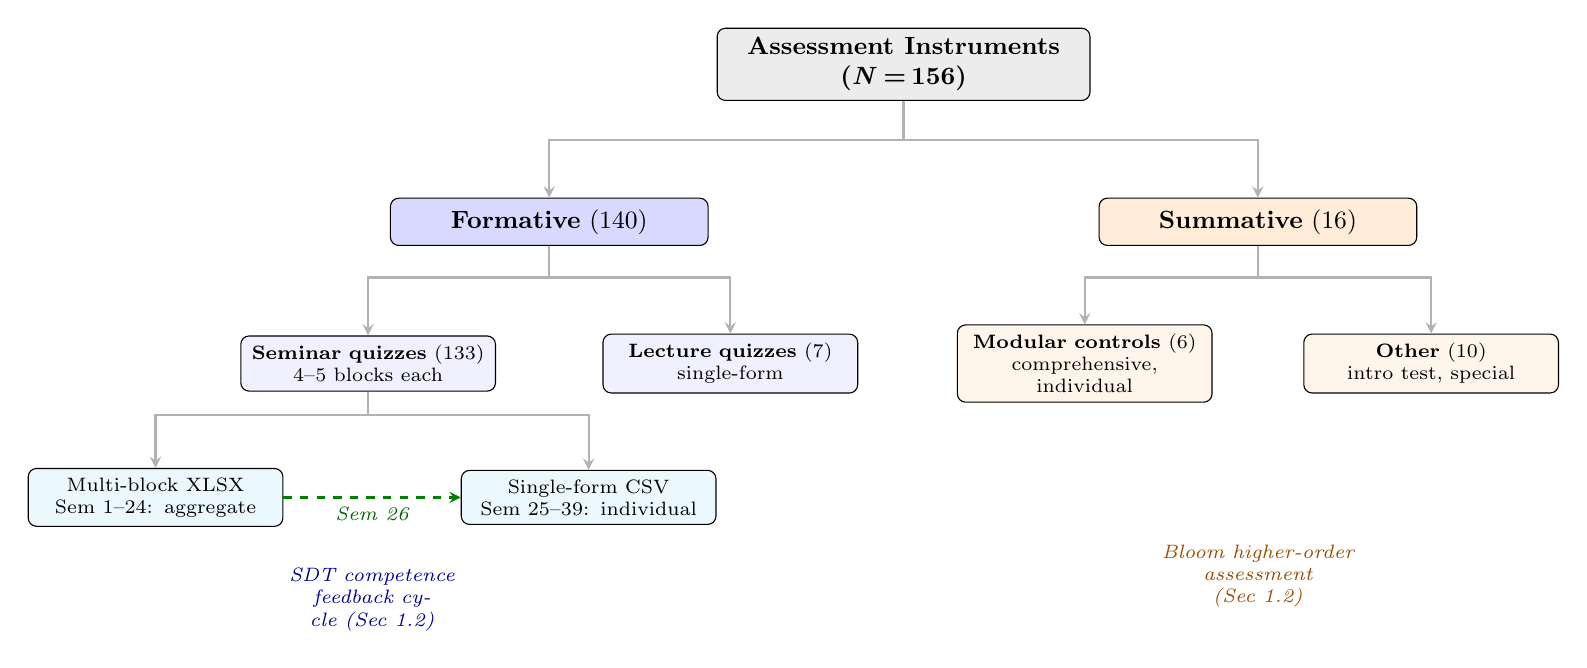
\begin{tikzpicture}[
  node distance=0.45cm,
  rootbox/.style={rectangle, draw, rounded corners=3pt, fill=gray!15,
    text width=4.5cm, minimum height=0.7cm, align=center, font=\small\bfseries},
  formbox/.style={rectangle, draw, rounded corners=3pt, fill=blue!15,
    text width=3.8cm, minimum height=0.6cm, align=center, font=\small},
  summbox/.style={rectangle, draw, rounded corners=3pt, fill=orange!15,
    text width=3.8cm, minimum height=0.6cm, align=center, font=\small},
  leafbox/.style={rectangle, draw, rounded corners=3pt, fill=white,
    text width=3.0cm, minimum height=0.5cm, align=center, font=\scriptsize},
  annot/.style={font=\scriptsize\itshape, text width=2.5cm, align=center},
  arr/.style={->, >=stealth, thick, gray!60}
]

% Root
\node[rootbox] (root) at (0, 0) {Assessment Instruments\\(\textit{N}\,=\,156)};

% Level 1: Formative / Summative — increased vertical gap
\node[formbox] (form) at (-4.5, -2.0) {\textbf{Formative} (140)};
\node[summbox] (summ) at (4.5, -2.0) {\textbf{Summative} (16)};

\draw[arr] (root.south) -- ++(0,-0.5) -| (form.north);
\draw[arr] (root.south) -- ++(0,-0.5) -| (summ.north);

% Formative children — increased vertical gap
\node[leafbox, fill=blue!6] (semq) at (-6.8, -3.8) {\textbf{Seminar quizzes} (133)\\{\scriptsize 4--5 blocks each}};
\node[leafbox, fill=blue!6] (lecq) at (-2.2, -3.8) {\textbf{Lecture quizzes} (7)\\{\scriptsize single-form}};

\draw[arr] (form.south) -- ++(0,-0.4) -| (semq.north);
\draw[arr] (form.south) -- ++(0,-0.4) -| (lecq.north);

% Seminar quiz sub-levels (data format evolution)
\node[leafbox, fill=cyan!8] (xlsx) at (-9.5, -5.5) {Multi-block XLSX\\{\scriptsize Sem 1--24: aggregate}};
\node[leafbox, fill=cyan!8] (csv) at (-4.0, -5.5) {Single-form CSV\\{\scriptsize Sem 25--39: individual}};

\draw[arr] (semq.south) -- ++(0,-0.3) -| (xlsx.north);
\draw[arr] (semq.south) -- ++(0,-0.3) -| (csv.north);

% Transition annotation
\draw[->, >=stealth, thick, green!50!black, dashed] (xlsx.east) -- node[below, font=\scriptsize\itshape, green!40!black] {Sem~26} (csv.west);

% Summative children — increased vertical gap
\node[leafbox, fill=orange!8] (mc) at (2.3, -3.8) {\textbf{Modular controls} (6)\\{\scriptsize comprehensive, individual}};
\node[leafbox, fill=orange!8] (other) at (6.7, -3.8) {\textbf{Other} (10)\\{\scriptsize intro test, special}};

\draw[arr] (summ.south) -- ++(0,-0.4) -| (mc.north);
\draw[arr] (summ.south) -- ++(0,-0.4) -| (other.north);

% Side annotations: placed BELOW the trees
\node[annot, text=blue!60!black] at (-6.75, -6.8) {SDT competence\\feedback cycle (Sec~1.2)};
\node[annot, text=orange!60!black] at (4.5, -6.5) {Bloom higher-order\\assessment (Sec~1.2)};

\end{tikzpicture}
}
\caption{Hierarchical taxonomy of assessment instruments (N=156), showing the formative--summative distinction and data format evolution from XLSX aggregate (Seminars~1--24) to CSV individual-level (Seminars~25--39)}
\label{fig:assessment-taxonomy}
\end{figure}

The quiz item design produces the score data that are analysed in Section~\ref{sec:formative}, where pre- and post-gamification performance patterns are compared.

\subsection{Creative quiz naming conventions} \label{sec:quiz-naming}

A distinctive feature of the course's gamification approach~\cite{Deterding2011, KoivistoHamari2019} was the use of creative, thematic naming for quiz blocks within each seminar. Rather than using generic labels (``Block 1'', ``Block 2''), the instructor adopted thematic naming schemes that changed with each seminar, creating an element of surprise and cultural enrichment~\cite{Sailer2017}. The naming themes included:

\begin{itemize}
\item \textbf{Gemstones}: Seminar 19 (Aметист/Amethyst, Берил/Beryl, Варисцит/Variscite, Геліодор/Heliodor)
\item \textbf{Greek mythology}: Seminar 20 (Ахіл/Achilles, Беллерофонт/Bellerophon, Скамандрій/Scamandrius, Діомед/Diomedes, Гектор/Hector)
\item \textbf{Greek alphabet}: Seminars 17, 21 (alpha, beta, gamma, delta, epsilon)
\item \textbf{Flowers}: Seminars 25, 29 (Айстра/Aster, Барвінок/Periwinkle, Волошка/Cornflower, Гіацинт/Hyacinth)
\item \textbf{Trees}: Seminar 27 (Акація/Acacia, Баобаб/Baobab, Вільха/Alder, Гінкго/Ginkgo)
\item \textbf{Minerals}: Seminar 30 (Азбест/Asbestos, Берил/Beryl, Воксит/Bauxite, Галіт/Halite)
\item \textbf{Roman numerals}: Seminar 8 (І, ІІ, ІІІ, IV, V)
\item \textbf{Chapter numbering}: Seminar 11 (Chapter 1--5)
\item \textbf{Simple numbering}: Various seminars (Блок 1--5)
\end{itemize}

This naming practice exemplifies \emph{content gamification}~\cite{SEABORN201514} --- the use of game-inspired framing to enhance the learning experience without altering the underlying assessment content~\cite{Titova2025cte, KorniienkoSemerikov2024}. In Landers'~\cite{Landers2014} theory of gamified learning, creative naming operates as a \emph{mediational} effect: the thematic framing enhances learner attitudes (engagement, curiosity), which in turn mediate learning behaviour and outcomes. Each naming theme creates a micro-narrative context, operationalising the narrative/theme design principle identified in Section~\ref{sec:principle-grounding} and illustrating how even minimal game elements can shift the affective experience of assessment. The parsed chat data (Section~\ref{sec:attendance}) confirm positive student reactions to the naming schemes, with participants occasionally referencing theme names in group discussion.

\subsection{Viber chat log as data source}

The Viber messenger group served as the primary communication channel for the course~\cite{Vovchasta2024}. Unlike researcher-constructed instruments (quizzes, surveys), the chat log constitutes an \emph{unobtrusive} data source~\cite{CohenManionMorrison2018}: messages were generated naturally as part of the course's operational communication, without any researcher prompting or structured elicitation. This naturalistic quality provides ecological validity that complements the structured quiz data.

\paragraph{Data collection protocol.}
The chat log was exported in plain text format from Viber, preserving timestamps (date, time), sender names, and message content. Automated parsing (Section~\ref{sec:organisation}) extracted 400~structured messages over the study period October~12, 2024 -- May~11, 2025. Participant names were anonymised using a deterministic hashing procedure to enable individual tracking while protecting privacy.

\paragraph{Data categories.}
The chat data provided six categories of information:

\begin{itemize}
\item \textbf{Enrollment timeline}: 28 join events for 23 unique participants (some joined multiple times after being removed and re-added);
\item \textbf{Absence reports}: 33 messages reporting inability to attend, with classified reasons (internet 24\%, family 24\%, unspecified 24\%, power 9\%, health 9\%, late 9\%);
\item \textbf{Assessment links}: All 156 Google Forms links shared during the course, verified against the quiz exports;
\item \textbf{Teaching materials}: 51 file shares (worksheets, presentations) and 46 video shares (lecture recordings);
\item \textbf{Gamification introductions}: Links to HistoryLikeGame platform (December 1, 2024; December 29, 2024) and Wordwall (March 27, 2025);
\item \textbf{Wartime context}: Messages about power outages, internet disruptions, air raid alerts, and safety advisories~\cite{Martynets202428, UNESCO2023}.
\end{itemize}

\paragraph{Data integrity.}
The 400~parsed messages represent the methodologically relevant subset of total group communication. All 156~quiz links were cross-verified against Google Forms exports to ensure completeness. The chat data feed three distinct analyses in Chapter~3: enrollment dynamics (Figure~\ref{fig:enrollment}), attendance patterns (Section~\ref{sec:attendance}), and the assessment timeline.

Figure~\ref{fig:data-matrix} presents the data collection matrix, mapping data types to study phases and indicating the level of granularity available in each cell.

\begin{figure}[htbp]
\centering
\resizebox{\textwidth}{!}{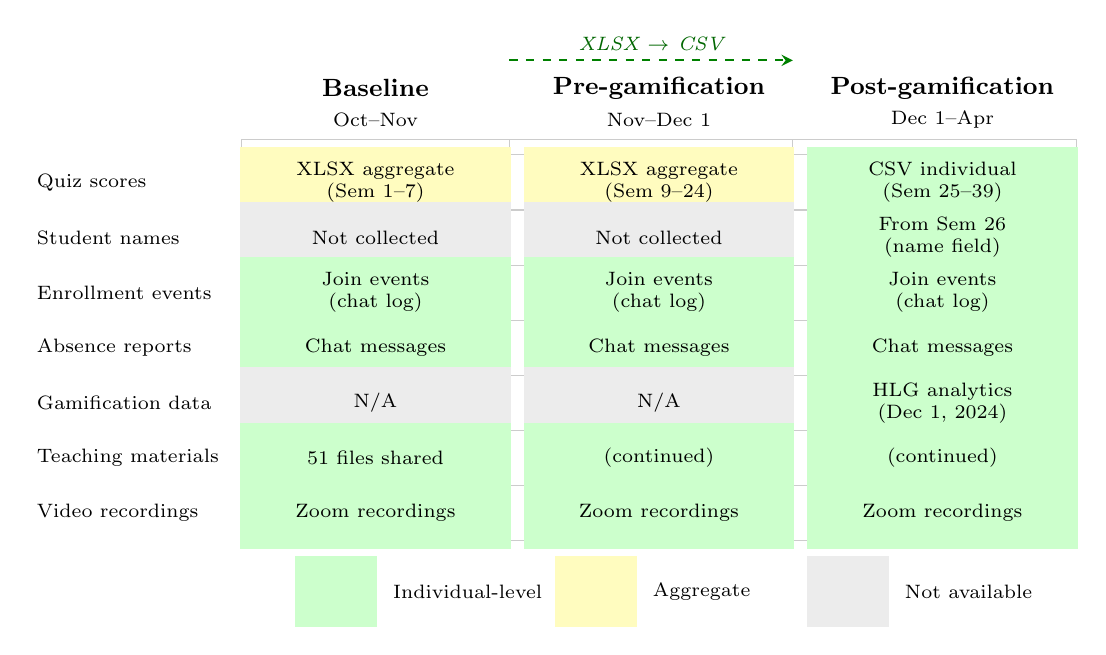
\begin{tikzpicture}[
  font=\small,
  cell/.style={minimum width=3.4cm, minimum height=0.9cm, align=center, font=\scriptsize, text width=3.2cm},
  indiv/.style={cell, fill=green!20},
  aggr/.style={cell, fill=yellow!25},
  nodata/.style={cell, fill=gray!15},
  header/.style={minimum width=3.4cm, minimum height=0.5cm, align=center, font=\small\bfseries, fill=white},
  subheader/.style={minimum width=3.4cm, minimum height=0.4cm, align=center, font=\scriptsize, fill=white},
  rowlabel/.style={minimum width=2.8cm, minimum height=0.7cm, align=left, font=\scriptsize, text width=2.6cm},
  phasearr/.style={->, >=stealth, thick, green!50!black, dashed}
]

% Column positions: row labels at x=1.0, columns at x=4.0, 7.6, 11.2
\def\cola{4.0}
\def\colb{7.6}
\def\colc{11.2}
\def\rowx{1.0}

% Column headers (two rows: title + date range)
\node[header] at (\cola, 0.2) {Baseline};
\node[subheader] at (\cola, -0.2) {Oct--Nov};
\node[header] at (\colb, 0.2) {Pre-gamification};
\node[subheader] at (\colb, -0.2) {Nov--Dec 1};
\node[header] at (\colc, 0.2) {Post-gamification};
\node[subheader] at (\colc, -0.2) {Dec 1--Apr};

% Row labels and horizontal lines
\foreach \y/\rowlbl in {
  -1.0/Quiz scores,
  -1.7/Student names,
  -2.4/Enrollment events,
  -3.1/Absence reports,
  -3.8/Gamification data,
  -4.5/Teaching materials,
  -5.2/Video recordings%
}{
  \node[rowlabel] at (\rowx, \y) {\rowlbl};
  \draw[gray!40] (2.3, \y+0.35) -- (12.9, \y+0.35);
}
\draw[gray!40] (2.3, -0.45) -- (12.9, -0.45);
\draw[gray!40] (2.3, -5.55) -- (12.9, -5.55);

% Vertical dividers
\foreach \x in {2.3, 5.7, 9.3, 12.9}{
  \draw[gray!40] (\x, -0.45) -- (\x, -5.55);
}

% Quiz scores row
\node[aggr] at (\cola, -1.0) {XLSX aggregate\\(Sem 1--7)};
\node[aggr] at (\colb, -1.0) {XLSX aggregate\\(Sem 9--24)};
\node[indiv] at (\colc, -1.0) {CSV individual\\(Sem 25--39)};

% Student names row
\node[nodata] at (\cola, -1.7) {Not collected};
\node[nodata] at (\colb, -1.7) {Not collected};
\node[indiv] at (\colc, -1.7) {From Sem 26\\(name field)};

% Enrollment row
\node[indiv] at (\cola, -2.4) {Join events\\(chat log)};
\node[indiv] at (\colb, -2.4) {Join events\\(chat log)};
\node[indiv] at (\colc, -2.4) {Join events\\(chat log)};

% Absence row
\node[indiv] at (\cola, -3.1) {Chat messages};
\node[indiv] at (\colb, -3.1) {Chat messages};
\node[indiv] at (\colc, -3.1) {Chat messages};

% Gamification row
\node[nodata] at (\cola, -3.8) {N/A};
\node[nodata] at (\colb, -3.8) {N/A};
\node[indiv] at (\colc, -3.8) {HLG analytics\\(Dec 1, 2024)};

% Materials row
\node[indiv] at (\cola, -4.5) {51 files shared};
\node[indiv] at (\colb, -4.5) {(continued)};
\node[indiv] at (\colc, -4.5) {(continued)};

% Video row
\node[indiv] at (\cola, -5.2) {Zoom recordings};
\node[indiv] at (\colb, -5.2) {Zoom recordings};
\node[indiv] at (\colc, -5.2) {Zoom recordings};

% Data format evolution arrow — placed above column headers
\draw[phasearr] (5.7, 0.55) -- node[above, font=\scriptsize\itshape, green!40!black] {XLSX $\to$ CSV} (9.3, 0.55);

% Legend
\node[indiv, minimum width=1.0cm, text width=0.8cm] at (3.5, -6.2) {};
\node[font=\scriptsize, anchor=west] at (4.1, -6.2) {Individual-level};
\node[aggr, minimum width=1.0cm, text width=0.8cm] at (6.8, -6.2) {};
\node[font=\scriptsize, anchor=west] at (7.4, -6.2) {Aggregate};
\node[nodata, minimum width=1.0cm, text width=0.8cm] at (10.0, -6.2) {};
\node[font=\scriptsize, anchor=west] at (10.6, -6.2) {Not available};

\end{tikzpicture}
}
\caption{Data collection matrix: data types (rows) mapped to study phases (columns). Green = individual-level data, yellow = aggregate data, gray = not available. The XLSX-to-CSV transition marks the shift from aggregate to individual-level quiz score data.}
\label{fig:data-matrix}
\end{figure}

\subsection{Scoring, feedback, and data quality} \label{sec:scoring}

\paragraph{Scoring procedure.}
Quiz scores were generated automatically by Google Forms' built-in scoring engine. Each item was assigned a point value, and the total score was reported in the ``X~/~Y'' string format (achieved~/~maximum). For modular controls, a hybrid approach was used: objective items (multiple choice, matching) were auto-scored, while open-ended items were manually graded by the instructor. Score data were exported in two formats depending on the period: multi-sheet XLSX files (Seminars~1--24) containing aggregate statistics, and single-sheet CSV files (Seminars~25--39) containing individual-level responses.

\paragraph{Feedback timing and theoretical grounding.}
All quizzes provided immediate feedback upon submission --- students saw their score within seconds of completing the form. In Hattie and Timperley's~\cite{HattieTimperley2007} four-level feedback model, this operates primarily at the \emph{task level} (correctness of response) and \emph{process level} (strategies used to approach the task). The immediate delivery satisfies the SDT competence need~\cite{RyanDeci2000} (Section~\ref{sec:theory}) by providing timely information about one's effectiveness, and constitutes one of the preconditions for flow states~\cite{Csikszentmihalyi1990}. Van der Kleij et al.'s~\cite{VanDerKleij2015} meta-analysis of feedback in computer-based environments supports the effectiveness of immediate elaborated feedback for procedural knowledge tasks, which characterises the majority of the quiz items in this study. This aligns with the broader assessment-in-game-based-learning framework proposed by Ifenthaler et al.~\cite{IfenthalerEseryel2012}, who argue that embedded assessment should be unobtrusive and aligned with the learning activity itself.

\paragraph{Score normalisation.}
The maximum possible scores varied substantially across seminars (range: 5--131 points), reflecting differences in the number of items and topic complexity. To enable cross-seminar comparison, all raw scores were normalised to percentages ($\text{score}_\% = X / Y \times 100$). The normalisation procedure and its statistical implications are detailed in Section~\ref{sec:data-analysis}.

\paragraph{Data completeness and respondent progression.}
Figure~\ref{fig:respondent-progression} presents the number of respondents per seminar across the full study period. Respondent counts ranged from 1 (Seminars~28, 30) to 27 (Seminar~17), with a marked decline in the post-gamification period. The mean number of respondents was $\bar{N}=12.9$ in the pre-gamification period (Seminars~1--24) versus $\bar{N}=5.6$ in the post-gamification period (Seminars~25--39). This decline is attributable primarily to natural attrition in a voluntary preparatory course and the increasing difficulty of later historical periods, rather than to gamification effects (see Section~\ref{sec:discussion} for a full discussion of confounding factors).

\begin{figure}[htbp]
\centering
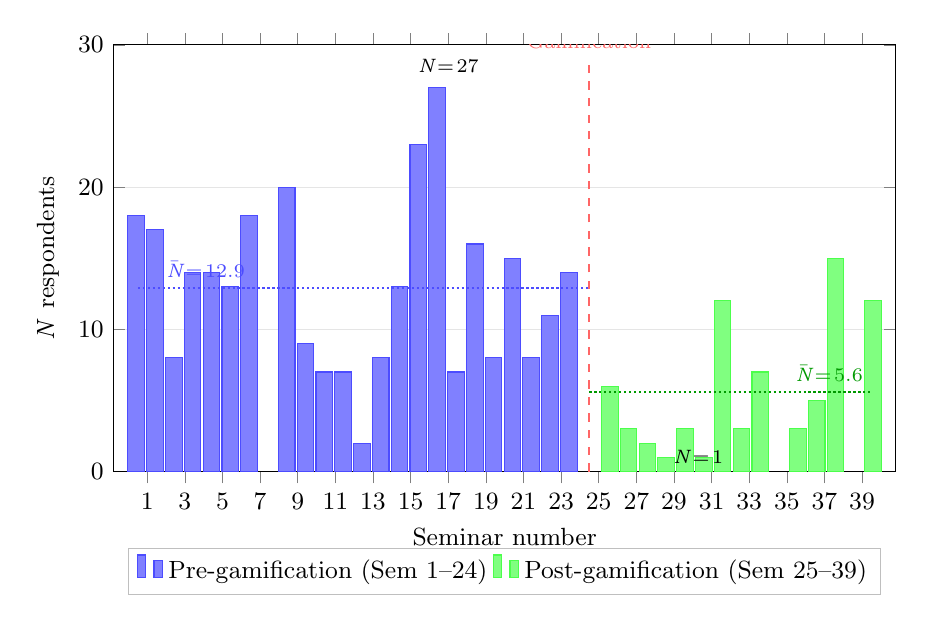
\begin{tikzpicture}
\begin{axis}[
  ybar,
  width=0.95\textwidth,
  height=7cm,
  bar width=6pt,
  ylabel={\textit{N} respondents},
  xlabel={Seminar number},
  ymin=0, ymax=30,
  xtick={1,3,5,7,9,11,13,15,17,19,21,23,25,27,29,31,33,35,37,39},
  xmin=0, xmax=40,
  enlarge x limits=0.02,
  legend style={at={(0.5,-0.18)}, anchor=north, legend columns=2, font=\small, draw=gray!50},
  ymajorgrids=true,
  grid style={gray!20},
  tick label style={font=\small},
  label style={font=\small},
]

% Pre-gamification bars (blue)
\addplot[fill=blue!50, draw=blue!70] coordinates {
  (1,18) (2,17) (3,8) (4,14) (5,14) (6,13) (7,18)
  (9,20) (10,9) (11,7) (12,7) (13,2) (14,8) (15,13)
  (16,23) (17,27) (18,7) (19,16) (20,8) (21,15) (22,8) (23,11) (24,14)
};

% Post-gamification bars (green)
\addplot[fill=green!50, draw=green!70] coordinates {
  (25,6) (26,3) (27,2) (28,1) (29,3) (30,1)
  (31,12) (32,3) (33,7) (35,3) (36,5) (37,15) (39,12)
};

\legend{Pre-gamification (Sem 1--24), Post-gamification (Sem 25--39)}

% Gamification boundary
\draw[dashed, thick, red!60] (axis cs:24.5,0) -- (axis cs:24.5,29)
  node[above, font=\scriptsize, red!60] {Gamification};

% Period mean lines
\draw[densely dotted, blue!70, thick] (axis cs:0.5,12.9) -- (axis cs:24.5,12.9)
  node[pos=0.15, above, font=\scriptsize, blue!70] {$\bar{\textit{N}}\!=\!12.9$};
\draw[densely dotted, green!60!black, thick] (axis cs:24.5,5.6) -- (axis cs:39.5,5.6)
  node[pos=0.85, above, font=\scriptsize, green!60!black] {$\bar{\textit{N}}\!=\!5.6$};

% Annotations
\node[font=\scriptsize, above, yshift=2pt] at (axis cs:17,27) {$\textit{N}\!=\!27$};
\node[font=\scriptsize, right, xshift=3pt] at (axis cs:28,1) {$\textit{N}\!=\!1$};

\end{axis}
\end{tikzpicture}

\caption{Number of respondents per seminar quiz. Blue bars = pre-gamification period (Seminars~1--24, $\bar{N}=12.9$); green bars = post-gamification period (Seminars~25--39, $\bar{N}=5.6$). Dashed vertical line marks the gamification introduction (December~1, 2024).}
\label{fig:respondent-progression}
\end{figure}

\paragraph{Participant identification.}
The anonymous early seminars (1--25) limit analysis to aggregate statistics, while the name field introduced from Seminar~26 enables individual trajectory tracking for the post-gamification period. This creates a data discontinuity: individual-level analyses (Section~\ref{sec:formative}) are restricted to Seminars~26--39, where 90~named participants contributed 358~data points. The design implications of this discontinuity --- and the deliberate decision to introduce it mid-course --- are discussed as a design-based research iteration in Section~\ref{sec:organisation}.

The processing of these raw data sources into analytical outputs is detailed in Section~\ref{sec:data-analysis}.

\section{Gamification design: the HistoryLikeGame platform} \label{sec:gamification-design}

\subsection{Platform overview}

HistoryLikeGame is an interactive web-based gamification platform developed specifically for this study~\cite{KorniienkoSemerikov2024, Titova2025cte}. The platform is hosted at \texttt{astrafreeman.github.io/HistoryLikeGame/} and employs a hub-and-spoke architecture: a central index page (Figure~\ref{fig:hlg-hub}) links to 62 interactive game modules spanning 9 historical periods, implemented using a shared CSS/JavaScript infrastructure layer ($\approx$88~KB) that provides consistent theming, navigation, accessibility controls, and game engine logic across all modules~\cite{Zainuddin20241261, Uskov2015}. The platform requires no software installation, account creation, or server-side processing, functioning entirely as client-side static HTML/CSS/JavaScript that can be accessed from any device with a web browser. An animated octopus assistant provides historical facts and navigational guidance throughout the platform.

\begin{figure}[htbp]
\centering

\includegraphics[width=0.75\textwidth]{hlg_hub.png}
\caption{HistoryLikeGame platform hub page showing the 9 historical period cards, AR game section, embedded mini-game ($\beta$), and the octopus assistant mascot}
\label{fig:hlg-hub}
\end{figure}

\subsection{Platform evolution} \label{sec:platform-evolution}

The HistoryLikeGame platform underwent significant expansion during and after the study period. The experimental version~(v1), deployed on December~1, 2024, comprised 23 quiz modules organised into 5~sections plus an Omega comprehensive review, with a total code size of 205~KB. These modules used two interaction types: drag-and-drop matching and text input. The experimental data reported in Chapter~\ref{ch:results} are based exclusively on this version.

The current version~(v2), completed after the experimental period, expanded the platform to 62 modules across 9 historical periods plus bonus sections, incorporating 13~distinct game types including quiz-based exercises, Canvas physics games, Three.js 3D environments, card and board games, simulation, and AR experiences. The shared infrastructure layer was extracted and modularised ($\approx$88~KB of reusable CSS and JavaScript), accessibility features were added (theme switching, font scaling, motion reduction, high contrast), and documentation was provided for both players and developers. This chapter describes the current version~(v2) as it represents the practical contribution at the time of defence; Chapter~\ref{ch:results} specifies the experimental version where relevant.

\paragraph{Predecessor context.}
The HistoryLikeGame platform was not the first gamification attempt within the course. An earlier prototype, ``\foreignlanguage{ukrainian}{100 ігор з історії}'' [100 Games in History] (preserved in the repository as \texttt{cite\_structure/}), employed a monolithic single-page architecture with embedded game sections and an animated octopus assistant. While this prototype demonstrated the feasibility of browser-based historical gamification, its limitations --- single-page architecture preventing modular navigation, no shared infrastructure layer, limited scalability beyond the initial game set --- motivated the hub-and-spoke redesign that became HistoryLikeGame. In design-based research terms~\cite{Adams2022119, WangHannafin2005}, this prototype constitutes Phase~0: a proof-of-concept whose practical shortcomings informed the subsequent design iterations.

\paragraph{Three-phase DBR narrative.}
The platform evolution can be structured as three design-based research iterations~\cite{Bakker2018}, each responding to limitations revealed by the preceding phase:
\begin{itemize}
\item \emph{Phase~0} (pre-experiment): The \texttt{cite\_structure} prototype --- monolithic, with limited game-type diversity and no modular infrastructure. Revealed that a single-page approach cannot scale to cover multiple historical periods with diverse interaction types.
\item \emph{Phase~1} (experimental, December~1, 2024): HistoryLikeGame~v1 --- 23 quiz modules, 2 interaction types (drag-and-drop, text input), 205~KB total. Validated that quiz-based gamification engages NMT preparatory learners, but demonstrated the need for broader modality coverage beyond recognition and recall tasks.
\item \emph{Phase~2} (post-experimental): HistoryLikeGame~v2 --- 62 modules, 13 game types, extracted shared infrastructure (8~JavaScript modules: \texttt{accessibility.js}, \texttt{assistant.js}, \texttt{canvas-utils.js}, \texttt{game-engine.js}, \texttt{nav.js}, \texttt{quiz-engine.js}, \texttt{ui-utils.js}; 6~CSS files: \texttt{reset.css}, \texttt{theme.css}, \texttt{layout.css}, \texttt{components.css}, \texttt{animations.css}, \texttt{responsive.css}). Generalised infrastructure enables rapid addition of new game types and periods.
\end{itemize}
This iterative trajectory exemplifies the DBR principle that ``each iteration successively approximated the ideal''~\cite{Bakker2018}: each phase produced both a functional artefact and design knowledge that shaped the next iteration. The overall DBR framing of the study is described in Section~\ref{sec:organisation}.

\subsection{Structure and content}

The platform comprises 62 game modules organised into 9 historical periods plus bonus sections (Table~\ref{tab:game-modules}), reflecting the principle of progressive difficulty~\cite{Clark2016, Connolly2012}. The period structure mirrors the chronological organisation of the NMT curriculum from ancient times to Ukrainian independence:

\begin{table}[htbp]
\centering
\caption{Structure of the HistoryLikeGame platform (current version)}
\label{tab:game-modules}
\small
\begin{tabular}{clcl}
\hline
\textbf{Period} & \textbf{Name} & \textbf{Modules} & \textbf{Game types} \\
\hline
0 & Introduction & 4 & Chronobiy, Block Buster, Compass, Solitaire \\
1 & Ancient history & 1 & Interactive path builder \\
2 & Rus-Ukraine & 2 & Falling-answer quiz, Apple catcher \\
3 & Grand Duchy of Lithuania & 1 & Falling-answer quiz \\
4 & Cossack era & 2 & Historical solitaire, Falling-answer \\
5 & Imperial period & 2 & Bobble shooter, Tower defence \\
6 & Ukrainian Revolution & 1 & Wordwall integration \\
7 & Soviet period & 1 & Portrait puzzle \\
8 & Independence & 1 & Caf\'{e} simulator \\
$\alpha$ & Christmas special & 23 & Quiz (D\&D + text input) \\
$\beta$ & Mini-game & 1 & Inline puzzle \\
AR & Augmented reality & 3+ & A-Frame 3D scenes \\
\hline
\multicolumn{2}{l}{\textbf{Total}} & \textbf{62} & \\
\hline
\end{tabular}
\end{table}

The distribution of modules reflects both the breadth of each historical period and the diversity of game types employed. Period~0 (Introduction) serves as an orientation section offering four distinct game types that collectively introduce the core historical timeline from Kyivan Rus to Ukrainian independence. The Christmas special section~($\alpha$, comprising the original 23 quiz modules from the experimental period) uses a grid-based unlock system with password progression. Each period-specific module employs a game type suited to its content: the Cossack era features a historical solitaire card game (Figure~\ref{fig:hlg-solitaire}), the Imperial period uses a bobble shooter with colour-coded historical categories, and the Soviet period employs a portrait puzzle with drag-and-drop fragments of historical figures. The complete per-module catalogue appears in Appendix~B (Table~\ref{tab:game-catalog}).

\subsection{Game types and interaction design}

Automated analysis of the platform modules (using the \texttt{catalog\_gamification.py} module of the data pipeline) identified six categories of game types with distinct cognitive demands and technological implementations~\cite{Prensky2001, Clark2016, Knutas2016}:

\begin{enumerate}
\item \textbf{Quiz-based} (23 modules in the $\alpha$ section): Drag-and-drop matching and text input exercises using the shared quiz engine. Drag-and-drop engages recognition memory and spatial reasoning~\cite{Bonwell1991, Qian2016, Lampropoulos2024}, while text input requires active recall for dates, names, and terminology~\cite{Connolly2012, Clark2016}. Figure~\ref{fig:hlg-quiz} shows a representative quiz module.
\item \textbf{Canvas physics games} (5 modules): Block Buster (breakout/arkanoid), bobble shooter (Figure~\ref{fig:hlg-bobble}), apple catcher, compass navigation, and falling-answer quizzes. These use HTML5 Canvas for real-time physics simulation, requiring timing and spatial coordination alongside historical knowledge.
\item \textbf{Three.js 3D environments} (2 modules): Chronobiy (Figure~\ref{fig:hlg-threejs}), a timeline-sorting battle game, and tower defence use Three.js for 3D rendering of historical scenarios with interactive gameplay.
\item \textbf{Card and board games} (2 modules): Historical solitaire (Figure~\ref{fig:hlg-solitaire}) where cards represent events within thematic categories (Hetman politics, Military campaigns, Cultural life, International relations) that must be sorted chronologically. A separate introductory solitaire provides general practice.
\item \textbf{Simulation and navigation} (3 modules): A caf\'{e} simulator set in the Independence period, a path-builder for ancient history, and a Wordwall-integrated revolution quiz. These employ varied interaction models from resource management to external platform embedding.
\item \textbf{AR experiences} (3+ modules): Augmented reality scenes using A-Frame and AR.js, including Quebec, Toronto, and Yukon variants with 3D model interaction. These require a camera-equipped device and represent the highest infrastructure tier~\cite{1Barbatsis201159}.
\end{enumerate}

The technical characteristics of each game type category are summarised in Table~\ref{tab:game-detail}.

\begin{table}[htbp]
\centering
\caption{Technical characteristics of HistoryLikeGame game type categories}
\label{tab:game-detail}
\small
\begin{tabular}{lccp{4.5cm}}
\hline
\textbf{Game type} & \textbf{Modules} & \textbf{Technology} & \textbf{Interaction model} \\
\hline
Quiz (D\&D + text) & 23 & Shared quiz engine & Drag-and-drop matching, text recall \\
Falling-answer & 3 & Shared game engine & Timed selection of falling items \\
Canvas physics & 5 & HTML5 Canvas & Real-time physics, spatial coordination \\
Three.js 3D & 2 & Three.js & 3D timeline sorting, tower defence \\
Card/board & 2 & Canvas/DOM & Chronological card sorting by theme \\
Simulation & 3 & Canvas/DOM/Wordwall & Resource management, path building \\
AR experiences & 3+ & A-Frame + AR.js & 3D model interaction via camera \\
Puzzle & 1 & DOM drag-and-drop & Portrait fragment assembly \\
\hline
\multicolumn{2}{l}{\textbf{Total modules}} & \textbf{62} & \\
\hline
\end{tabular}
\end{table}

\paragraph{Game type--competency mapping.}
Each game type was selected to target specific NMT competencies at defined cognitive levels (Bloom's revised taxonomy):
\begin{itemize}
\item \emph{Quiz (drag-and-drop + text input)}: Factual recall and term--definition matching $\rightarrow$ Remember and Understand;
\item \emph{Falling-answer}: Timed chronological selection under time pressure $\rightarrow$ Remember (procedural fluency);
\item \emph{Canvas physics}: Spatial reasoning applied to historical content (breakout, bobble shooter) $\rightarrow$ Apply;
\item \emph{Three.js 3D}: Chronological sorting within immersive 3D environments $\rightarrow$ Analyse;
\item \emph{Card/board}: Thematic categorisation of events across multiple dimensions $\rightarrow$ Analyse and Evaluate;
\item \emph{Simulation}: Resource management and decision-making in historical scenarios $\rightarrow$ Evaluate and Create;
\item \emph{AR experiences}: Spatial interaction with 3D historical models $\rightarrow$ Apply (novel modality).
\end{itemize}
This mapping extends the platform type $\times$ pedagogical affordance analysis from Section~\ref{sec:game-elements} (Figure~\ref{fig:platform-pedagogy-matrix}), where web-based platforms scored ``Strong'' on assessment integration, scalability, and cost-effectiveness --- directly justifying the HTML5/JavaScript technology choice. The progression from recognition-level quiz tasks to synthesis-level simulation mirrors the progressive complexity principle~\cite{Clark2016, Connolly2012}.

The shared infrastructure layer --- comprising 6~CSS files ($\approx$28~KB), 8~JavaScript modules ($\approx$49~KB), and 2~HTML templates ($\approx$11~KB) --- totals approximately 88~KB and is reused across all modules. The total platform code (HTML+CSS+JS) is approximately 869~KB, while data files (quiz questions, game configurations, assistant facts) add $\approx$1.5~MB, and multimedia assets (images, 3D models, audio) bring the full platform to approximately 76~MB. For the code-only portion, the platform remains exceptionally lightweight compared to other educational technology platforms~\cite{Zainuddin20241261}: the shared infrastructure layer that powers all game types is smaller than a single lecture slide image. This size advantage is critical in the wartime context, where bandwidth limitations frequently affect educational access~\cite{Martynets202428, Vovchasta2024}. The per-module catalogue with individual sizes appears in Appendix~B (Table~\ref{tab:game-catalog}).

Each module provides immediate visual feedback upon interaction, using colour coding (green for correct, red for incorrect) and score tracking~\cite{Hattie2009}. The feedback mechanism aligns with the ``immediate feedback'' design principle identified in the systematic review (Section~\ref{sec:gamification-review})~\cite{KorniienkoSemerikov2024}.

\subsection{Design rationale}

The platform's design was guided by the principles identified in Section~\ref{sec:gamification-review}~\cite{KorniienkoSemerikov2024, Korniienko2025aredu}:

\begin{itemize}
\item \textbf{Historical authenticity}: All content was based on the NMT curriculum and verified historical facts~\cite{KorniienkoSemerikov2024, Christiansson200593};
\item \textbf{Progressive complexity}: Periods follow the chronological structure of the course, from ancient history through independence, with the $\alpha$ section's Omega module providing a comprehensive challenge~\cite{Clark2016, Hamari2014, Laskowski2015};
\item \textbf{Inclusivity and accessibility}: The platform implements inclusive design through a floating settings panel (Figure~\ref{fig:hlg-accessibility}) that provides theme switching (dark/light), font size scaling (A/A+/A++), motion reduction, and high-contrast mode --- accommodating diverse visual preferences, motor abilities, and sensory sensitivities~\cite{McCrindle2013}. All settings persist via \texttt{localStorage} and respect system-level preferences (\texttt{prefers-color-scheme}, \texttt{prefers-reduced-motion}, \texttt{prefers-contrast}). Static HTML delivery ensures minimal bandwidth requirements and universal device compatibility~\cite{Vuorikari2016, Zainuddin20241261};
\item \textbf{Offline capability}: Once loaded, all game modules function entirely without network connectivity, as no server communication is required after initial page load. This is critical in the wartime context where internet connectivity is unreliable~\cite{Martynets202428, Vovchasta2024};
\item \textbf{Immediate feedback}: Instant visual feedback (colour-coded green/red responses, score tracking) supports self-regulated learning~\cite{Hattie2009, Connolly2012};
\item \textbf{Low barrier to entry}: No registration, login, or software installation required~\cite{Prensky2001};
\item \textbf{Documentation}: Player and developer guides are provided in both HTML and Markdown formats, enabling educators to understand, adapt, and extend the platform.
\end{itemize}

\paragraph{Theoretical grounding of design decisions.}
Each design principle connects to an established theoretical framework identified in Chapter~1. Historical authenticity operationalises the disciplinary literacy approach, where game content must reflect genuine historical inquiry rather than trivialised narratives (Section~\ref{sec:principle-grounding}). Progressive complexity implements the challenge--skill balance central to Flow Theory~\cite{Csikszentmihalyi1990}: as learners progress through historical periods, both content difficulty and game mechanic complexity increase, maintaining the ``flow channel'' between boredom and anxiety. Inclusivity features (theme switching, font scaling, motion reduction, high contrast) operationalise the principle that gamified learning should be accessible ``regardless of gender, age, culture, experience or any disabilities''~\cite{McCrindle2013}. These features align with WCAG accessibility guidelines and DigComp Area~5 problem-solving competences~\cite{Vuorikari2016}, directly responding to the finding that accessibility barriers impede gamification adoption~\cite{Sunkara2024203, Gasca-Hurtado2021382}. Offline capability directly mitigates first-order (technical) barriers~\cite{Ertmer1999}, responding to the 40.5\% technical barrier rate identified in the systematic review (Figure~\ref{fig:barrier-frequency}). Immediate feedback combines behaviourist reinforcement with SDT competence need satisfaction~\cite{RyanDeci2000, Hattie2009}: colour-coded responses provide both extrinsic information and intrinsic competence signals. Low barrier to entry addresses second-order (attitudinal) barriers~\cite{Ertmer1999} by eliminating registration friction. Documentation supports the MRQS replicability standard~\cite{Korniienko2025mrqs}, enabling other researchers and educators to reproduce or adapt the platform.

\paragraph{MDA framework mapping.}
Following the Mechanics--Dynamics--Aesthetics framework~\cite{Hunicke2004} introduced in Section~\ref{sec:dmc-mapping}: the platform's \emph{mechanics} include drag-and-drop interaction, text input, physics collision detection, card sorting algorithms, and timer-based challenges. These mechanics generate \emph{dynamics} of score tracking, progressive unlock (the $\alpha$ section's password-gated grid), thematic grouping by historical period, and difficulty escalation. The intended \emph{aesthetics} --- the emotional responses experienced by learners --- encompass narrative engagement (period-based historical storytelling), challenge (progressive difficulty and timed elements), and discovery (exploring new game types across periods). This three-layer analysis ensures that low-level implementation decisions (mechanics) are traceable to the learning experience goals (aesthetics) through observable interaction patterns (dynamics).

\subsection{Alignment with design principles}

The HistoryLikeGame platform was designed to implement the six evidence-based design principles identified in the systematic review (Section~\ref{sec:gamification-review})~\cite{KorniienkoSemerikov2024}. Table~\ref{tab:principle-alignment} maps each principle to specific platform features.

\begin{table}[htbp]
\centering
\caption{Alignment of HistoryLikeGame platform with evidence-based design principles}
\label{tab:principle-alignment}
\small
\begin{tabular}{p{3cm}p{4cm}p{5.5cm}}
\hline
\textbf{Design principle} & \textbf{Platform feature} & \textbf{Evidence from review} \\
\hline
Historical authenticity~\cite{KorniienkoSemerikov2024} & All content verified against NMT curriculum; factual accuracy maintained & Studies with accurate content reported stronger outcomes; 10.8\% reporting negatives linked to trivialisation~\cite{Prieto-Andreu2024244} \\
\hline
Narrative integration~\cite{Sailer2017} & Period-based structure following Ukrainian history chronologically; thematic quiz naming; octopus assistant providing historical facts & Quest-based structures aligned with historical investigation; strongest effects on affective outcomes~\cite{KorniienkoSemerikov2024} \\
\hline
Progressive difficulty~\cite{Clark2016} & Nine historical periods from ancient to independence; increasing game complexity from quizzes to 3D environments; Omega comprehensive review & Scaffolded challenges from recognition to analysis to synthesis supported sustained engagement~\cite{PrietoAndreu202073} \\
\hline
Immediate feedback~\cite{Hattie2009} & Colour-coded responses (green/red); instant score display; game-mechanic feedback (physics collisions, card placements) & Enabled iterative learning cycles; particularly effective for factual recall~\cite{Zhonggen2019} \\
\hline
Social elements~\cite{Qian2016} & Viber group sharing; peer support; community naming & Collaborative structures showed more consistently positive effects than competition~\cite{Hamari2014} \\
\hline
Multiple modalities~\cite{Tamim2011} & 13 game types: quiz, Canvas physics, Three.js 3D, card games, simulation, AR, puzzle; visual + textual + spatial + kinesthetic elements & Multimodal engagement addressed diverse learning preferences~\cite{Connolly2012} \\
\hline
\end{tabular}
\end{table}

Table~\ref{tab:principle-alignment} maps the six design principles from the systematic review. In addition, Section~\ref{sec:guidelines} formulated eight implementation guidelines that operationalise these principles through the DigComp framework. Table~\ref{tab:guidelines-impl} traces each guideline to its specific implementation in the experimental design.

\begin{table}[htbp]
\centering
\caption{Implementation of Section~\ref{sec:guidelines} guidelines in the experimental design}
\label{tab:guidelines-impl}
\small
\begin{tabular}{p{0.5cm}p{3.2cm}p{4cm}p{4.5cm}}
\hline
\textbf{\#} & \textbf{Guideline} & \textbf{Implementation} & \textbf{Evidence} \\
\hline
1 & Clear learning objectives & NMT curriculum defines content; DigComp~2.0 areas frame digital competencies (Section~\ref{sec:organisation}) & 156 quizzes aligned to NMT format \\
\hline
2 & Progressive complexity & 9 historical periods from ancient to independence; Bloom's taxonomy scaffolding (Section~\ref{sec:game-elements}) & Game types progress: quiz $\to$ card $\to$ 3D $\to$ simulation \\
\hline
3 & Historical rigour & All content verified against NMT curriculum; factual accuracy maintained & 0\% content complaints in 400 Viber messages \\
\hline
4 & Multiple pathways & Required seminars + optional HLG modules + Omega comprehensive review & 62 modules across 13 game types \\
\hline
5 & Integrated assessment & Google Forms quizzes as both formative assessment and learning activities (Section~\ref{sec:assessment}) & Iterative mastery: e.g., Talash~D., 7 attempts \\
\hline
6 & Inclusivity, accessibility, resilience & Theme switching, font scaling, motion reduction, high contrast; offline-capable; $<$30~KB per page (Section~\ref{sec:gamification-design}) & Five-layer resilience architecture (Figure~\ref{fig:resilience-architecture}) \\
\hline
7 & Community through gamification & Creative quiz naming; Viber group sharing; thematic naming conventions (Section~\ref{sec:quiz-naming}) & 400 Viber messages; naming themes referenced by students \\
\hline
8 & Systematic documentation & Chat log, response files, platform source code, Python analysis pipeline preserved (Section~\ref{sec:data-analysis}) & Reproducible pipeline; all data in Appendix~B \\
\hline
\end{tabular}
\end{table}

\begin{figure}[htbp]
\centering

\includegraphics[width=0.65\textwidth]{hlg_quiz.png}
\caption{Quiz module interface (Christmas special, Section~$\alpha$): text input for dates, multiple-choice buttons for historical content, and image-based architectural style identification}
\label{fig:hlg-quiz}
\end{figure}

\begin{figure}[htbp]
\centering

\includegraphics[width=0.75\textwidth]{hlg_threejs.png}
\caption{Chronobiy (``Time Slayer'') game: a timeline-sorting battle where players arrange historical events chronologically to defeat period-specific opponents. Built with Three.js for 3D visual effects}
\label{fig:hlg-threejs}
\end{figure}

\begin{figure}[htbp]
\centering

\includegraphics[width=0.75\textwidth]{hlg_solitaire.png}
\caption{Historical solitaire: Cossack era card game with four thematic categories (Hetman politics, Military campaigns, Cultural life, International relations) requiring chronological sorting within each theme}
\label{fig:hlg-solitaire}
\end{figure}

\begin{figure}[htbp]
\centering

\includegraphics[width=0.65\textwidth]{hlg_bobble.png}
\caption{Bobble Shooter: Imperial period game where coloured bubbles represent historical categories (Culture, Politics, Economy, Military affairs) and players match three or more to clear the field}
\label{fig:hlg-bobble}
\end{figure}

\begin{figure}[htbp]
\centering

\includegraphics[width=0.55\textwidth]{hlg_accessibility.png}
\caption{Inclusivity settings panel of the HistoryLikeGame platform: theme switching (dark/light), font size scaling (A/A+/A++), reduced motion, and high-contrast mode. Settings persist via \texttt{localStorage} and respect system-level user preferences}
\label{fig:hlg-accessibility}
\end{figure}

\subsection{Supplementary gamification tools}

In addition to HistoryLikeGame, the course utilised multiple gamification modalities~\cite{Deterding2011, SEABORN201514}:
\begin{itemize}
\item \textbf{Wordwall}: An external interactive game platform, deployed for a single session on March~27, 2025 (Seminar~36, Period~6: Ukrainian Revolution). The embedded module (\texttt{viraska.html}) provided a matching exercise using Wordwall's visual interface. The pedagogical rationale for incorporating an external platform was twofold: it offered interaction modalities not available in HLG (timed competitive matching with animated feedback), and the deliberate platform diversity helps prevent gamification fatigue --- a risk identified in the literature for single-platform deployments~\cite{Lampropoulos2024, Bozic2024538}.

\item \textbf{Creative quiz naming}: As described in Section~\ref{sec:quiz-naming}, the systematic practice of assigning thematic, narrative-laden names to Google Forms quizzes transformed the assessment layer itself into a gamification element. This strategy applies the narrative integration principle (Section~\ref{sec:design-principles}) to non-game content: quiz titles such as ``Challenge of the Cossack Era'' or ``The Soviet Labyrinth'' frame each assessment as a quest rather than a test~\cite{Sailer2017}.

\item \textbf{Historical memes}: Occasional, non-systematic sharing of history-themed memes in the Viber chat group. These served a community-building function~\cite{Qian2016} rather than a formal pedagogical one. Unlike the structured gamification elements above, meme sharing was informal and not tracked quantitatively --- a deliberate choice to maintain the organic social dynamics of the learning community without instrumentalising every interaction.
\end{itemize}


\section{Wartime education context} \label{sec:wartime-context}

The unique wartime context of this study requires explicit documentation~\cite{UNESCO2023, Martynets202428}, both to contextualise the findings and to inform future research conducted under similar conditions.

\subsection{Impact of armed conflict on education}

Since Russia's full-scale invasion on February 24, 2022, Ukrainian educational institutions have operated under unprecedented conditions~\cite{Zamkova2023299, Vovchasta2024}. The Dnipropetrovsk Oblast, where Kryvyi Rih is located, has experienced regular missile and drone attacks targeting energy infrastructure, resulting in systematic disruptions to electricity supply and internet connectivity. During the study period (October 2024 -- May 2025), participants experienced:

\begin{itemize}
\item \textbf{Power outages}: Scheduled and unscheduled electricity cuts affecting the ability to participate in synchronous Zoom sessions~\cite{Martynets202428, Zamkova2023299}. Rolling blackout schedules were common during winter months (November--February), with some areas experiencing 4--8 hours of outage per day.
\item \textbf{Internet disruptions}: Loss of internet connectivity due to infrastructure damage, power outages affecting routers and ISP equipment, or network congestion during recovery periods~\cite{Vovchasta2024}.
\item \textbf{Air raid alerts}: Missile and drone attack warnings requiring evacuation to shelters, interrupting both live sessions and individual study. The instructor explicitly provided safety guidance: ``Your safety is the most important thing [...] if in doubt, go to a shelter.''
\item \textbf{Psychological stress}: The cumulative effect of ongoing conflict, displacement, loss of family members or acquaintances, and uncertainty about the future creating a chronic stress environment that affects cognitive performance and motivation~\cite{UNESCO2023, Zamkova2023299}.
\end{itemize}

\paragraph{Quantitative evidence from the course.}
The attendance log (Section~\ref{sec:attendance}) documents 33 absence notifications from 10 distinct participants. The breakdown by reported reason reveals: internet connectivity issues --- 8 (24.2\%), family circumstances --- 8 (24.2\%), unspecified --- 8 (24.2\%), power outages --- 3 (9.1\%), lateness --- 3 (9.1\%), and health --- 3 (9.1\%). Infrastructure-directly-attributable absences (internet + power) account for 11 cases (33.3\%), confirming that wartime infrastructure disruption is a primary barrier to participation. These data are analysed in full in Section~\ref{sec:attendance} (Table~\ref{tab:absence-reasons}, Figure~\ref{fig:absence}); here the focus is on the methodological implications for course design. The 33.3\% infrastructure-attributable rate aligns with the barrier distribution identified in the systematic review (Figure~\ref{fig:barrier-frequency}), where technical barriers constituted the largest category at 40.5\%.

\paragraph{Student voice.}
The chat log preserves representative participant communications documenting the lived reality of wartime education. Power disruptions were reported directly: ``\foreignlanguage{ukrainian}{В мене зникло світло}'' [My power went out]. Internet instability was a recurring theme: ``\foreignlanguage{ukrainian}{Дуже поганий інтернет}'' [Very bad internet]. Family circumstances --- which in the wartime context may encompass displacement, caregiving for relatives affected by conflict, or security concerns --- were cited formally: ``\foreignlanguage{ukrainian}{Буду відсутня за сімейними обставинами}'' [I will be absent due to family circumstances]. These reports illustrate the cascade effects described in the barrier interaction model (Figure~\ref{fig:barrier-interaction-model}): a single infrastructure failure (e.g., power outage) disables multiple educational layers simultaneously.

\subsection{Multi-channel resilience architecture}

To maintain educational continuity under these conditions~\cite{Hlianenko2024, Vovchasta2024}, the course adopted a five-layer resilience architecture, where each layer provided redundancy for the others:

\begin{enumerate}
\item \textbf{Synchronous layer (Zoom)}: Live lectures and discussions delivered via video conferencing. When the instructor's internet failed, sessions were rescheduled or replaced with asynchronous materials.
\item \textbf{Communication layer (Viber)}: The messaging platform served as the persistent communication backbone. Viber messages could be received and sent even during brief connectivity windows, and the platform's offline caching ensured that messages posted during outages were delivered once connectivity resumed.
\item \textbf{Content layer (Google Drive)}: All lecture materials, worksheets, and supplementary resources were stored on Google Drive and could be accessed asynchronously when connectivity was available. The Drive-based architecture meant that materials were available 24/7 regardless of whether the instructor was online.
\item \textbf{Assessment layer (Google Forms)}: Quiz links remained active and accessible at any time, allowing students to complete assessments when their individual connectivity allowed, rather than requiring simultaneous online presence~\cite{Hattie2009}.
\item \textbf{Gamification layer (HistoryLikeGame)}: The static HTML architecture of the platform (shared infrastructure: $\approx$88~KB; individual game pages typically under 30~KB each) meant that game modules could be loaded even on extremely slow connections~\cite{KorniienkoSemerikov2024, Titova2025cte}. Once loaded, the modules functioned entirely offline, requiring no further server communication. This made the gamification layer the most resilient component of the educational architecture, with graceful degradation: if multimedia assets failed to load, the core gameplay remained functional.
\end{enumerate}

This multi-channel approach demonstrated resilience through redundancy~\cite{Tamim2011}: when any single channel failed (instructor internet, student power outage), alternatives remained available. The asynchronous nature of most course components meant that temporary disruptions did not result in permanent loss of educational access~\cite{Hlianenko2024, Zamkova2023299}. Figure~\ref{fig:digital-platforms} illustrates the digital platform integration resources used in the course.

\begin{figure}[htbp]
\centering

\includegraphics[width=0.65\textwidth]{posibnyk_6_digital_platforms.jpg}
\caption{Digital platform integration poster (``Plug In. Log On.'') showing the ecosystem of digital tools used in the course, showing the ecosystem of digital tools integrated into the course methodology}
\label{fig:digital-platforms}
\end{figure}

\begin{figure}[htbp]
\centering
\resizebox{0.85\textwidth}{!}{% Five-layer resilience architecture diagram
% Label: fig:resilience-architecture
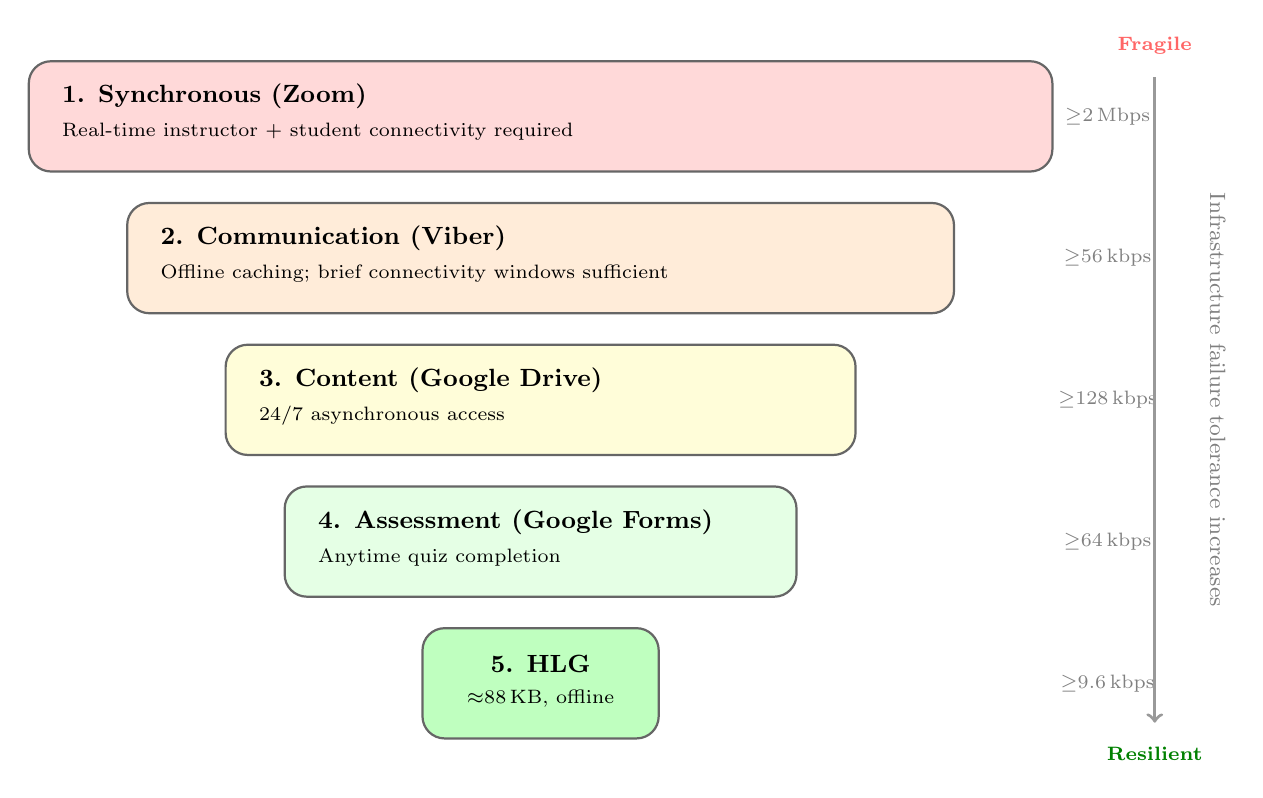
\begin{tikzpicture}[
  layer/.style={rounded corners=8pt, draw=black!60, line width=0.8pt, minimum width=#1, minimum height=1.4cm, align=center, font=\small},
  annot/.style={font=\footnotesize\itshape, text=black!70, align=left},
  bw/.style={font=\scriptsize, text=black!50, align=right}
]

% Layer 5 (outermost, most fragile) — Synchronous
\node[layer=13cm, fill=red!15] (L5) at (0, 0) {};
\node[font=\small\bfseries, anchor=west] at (-6.2, 0.25) {1. Synchronous (Zoom)};
\node[font=\scriptsize, anchor=west, text width=8cm] at (-6.2, -0.2) {Real-time instructor + student connectivity required};

% Layer 4 — Communication
\node[layer=10.5cm, fill=orange!15] (L4) at (0, -1.8) {};
\node[font=\small\bfseries, anchor=west] at (-4.95, -1.55) {2. Communication (Viber)};
\node[font=\scriptsize, anchor=west, text width=7cm] at (-4.95, -2.0) {Offline caching; brief connectivity windows sufficient};

% Layer 3 — Content
\node[layer=8cm, fill=yellow!15] (L3) at (0, -3.6) {};
\node[font=\small\bfseries, anchor=west] at (-3.7, -3.35) {3. Content (Google Drive)};
\node[font=\scriptsize, anchor=west, text width=5.5cm] at (-3.7, -3.8) {24/7 asynchronous access};

% Layer 2 — Assessment (widened from 5.5cm to 6.5cm)
\node[layer=6.5cm, fill=green!10] (L2) at (0, -5.4) {};
\node[font=\small\bfseries, anchor=west] at (-2.95, -5.15) {4. Assessment (Google Forms)};
\node[font=\scriptsize, anchor=west, text width=5cm] at (-2.95, -5.6) {Anytime quiz completion};

% Layer 1 (innermost, most resilient) — Gamification
\node[layer=3cm, fill=green!25] (L1) at (0, -7.2) {};
\node[font=\small\bfseries] at (0, -6.95) {5. HLG};
\node[font=\scriptsize] at (0, -7.4) {${\approx}$88\,KB, offline};

% Bandwidth annotations (right side)
\node[bw] at (7.2, 0) {$\geq$2\,Mbps};
\node[bw] at (7.2, -1.8) {$\geq$56\,kbps};
\node[bw] at (7.2, -3.6) {$\geq$128\,kbps};
\node[bw] at (7.2, -5.4) {$\geq$64\,kbps};
\node[bw] at (7.2, -7.2) {$\geq$9.6\,kbps};

% Arrow: failure tolerance increases
\draw[->, very thick, black!40] (7.8, 0.5) -- (7.8, -7.7);
\node[rotate=-90, font=\footnotesize, text=black!50] at (8.6, -3.6) {Infrastructure failure tolerance increases};

% Fragile/Resilient labels
\node[font=\scriptsize\bfseries, text=red!60] at (7.8, 0.9) {Fragile};
\node[font=\scriptsize\bfseries, text=green!50!black] at (7.8, -8.1) {Resilient};

\end{tikzpicture}
}
\caption{Five-layer resilience architecture of the course. Layers are ordered by infrastructure failure tolerance: outermost (synchronous Zoom) is most fragile; innermost (HistoryLikeGame, $\approx$88~KB, offline-capable) is most resilient. Bandwidth requirements decrease inward.}
\label{fig:resilience-architecture}
\end{figure}

\subsection{Implications for course design}

The wartime context informed six specific design decisions, each traceable to the resilience architecture described above:

\begin{enumerate}
\item \textbf{Asynchronous-first design.} All 40 lectures were recorded and shared via Google Drive (Layer~3), making synchronous attendance structurally optional rather than merely tolerated. This was necessary when real-time participation could not be guaranteed on any given day~\cite{Tamim2011, Hlianenko2024}. The overall course organisation reflecting this principle is described in Section~\ref{sec:organisation}.

\item \textbf{Voluntary formative assessment.} Seminar quizzes were voluntary, in contrast to mandatory modular controls, accommodating students whose participation was disrupted by infrastructure failures or safety concerns~\cite{Hickey2014}. The scoring rationale is detailed in Section~\ref{sec:scoring}.

\item \textbf{Minimal-bandwidth gamification.} The HistoryLikeGame platform's static HTML architecture (shared infrastructure $\approx$88~KB; individual pages typically $<$30~KB) was a deliberate design response to bandwidth constraints, not merely a technical convenience. The platform is loadable on 2G connections and functions entirely offline after initial load~\cite{KorniienkoSemerikov2024}. The platform evolution through three DBR iterations is described in Section~\ref{sec:platform-evolution}.

\item \textbf{Multi-channel redundancy.} The five-layer architecture (Figure~\ref{fig:resilience-architecture}) ensures that at least one educational pathway survives any single-point infrastructure failure~\cite{Vovchasta2024}. When the instructor's internet failed, Viber (Layer~2) provided scheduling updates; when students lost power, Google Drive materials (Layer~3) and offline HLG modules (Layer~5) remained accessible upon restoration.

\item \textbf{Safety-first communication.} The instructor's explicit guidance --- ``Your safety is the most important thing [\ldots] if in doubt, go to a shelter'' --- established a course culture prioritising student well-being over academic performance metrics~\cite{UNESCO2023}. This safety-first stance is documented in the chat log and analysed in Section~\ref{sec:attendance}.

\item \textbf{Rolling enrollment accommodation.} Late joiners had full access to all prior materials via Google Drive and could complete past assessments at their own pace. The asynchronous design imposed no penalty for late entry, an important consideration when displacement and infrastructure recovery timelines varied across participants~\cite{Zamkova2023299}. The enrollment patterns are analysed in Section~\ref{sec:baseline}.
\end{enumerate}


\section{Data analysis methods} \label{sec:data-analysis}

\subsection{Data processing pipeline}

A Python-based data processing pipeline was developed to systematically analyse all collected data~\cite{creswell, ary}. The pipeline addresses a key finding of the MRQS review (Section~\ref{sec:mrqs})~\cite{Korniienko2025mrqs}: the need for reproducible and transparent analytical procedures. By encoding all data processing steps in executable code, the pipeline ensures that analyses can be verified, replicated, and extended by other researchers~\cite{KitchenhamCharters2007}.

The pipeline consists of six sequential modules, each addressing a specific aspect of the data:

\begin{enumerate}
\item \textbf{Chat parser} (\texttt{parse\_chat.py}): Parses the 940-line Viber chat log into structured records~\cite{Thomas2008}. The parser uses regular expressions to handle Ukrainian date formats (e.g., ``13 жовтня 2024 р.'', ``1 березня 2025 р.'') and classifies each message into one of 15 categories: \texttt{join}, \texttt{leave}, \texttt{absence}, \texttt{seminar\_quiz}, \texttt{modular\_control}, \texttt{lecture\_quiz}, \texttt{intro\_test}, \texttt{gamification}, \texttt{file\_share}, \texttt{video\_share}, \texttt{announcement}, \texttt{safety}, \texttt{schedule}, \texttt{greeting}, and \texttt{other}. Output: \texttt{parsed\_chat.csv} with 400 classified messages.

\item \textbf{Assessment timeline extractor} (\texttt{extract\_assessments.py}): Builds a complete timeline of all 156 Google Forms quizzes from the parsed chat data~\cite{Page2021, Moher2009PRISMA, PageEtAl2021}. Each form is classified by type (seminar quiz: 133; lecture quiz: 7; modular control: 6; intro test: 1; other: 9) and associated with its seminar number, block name, date, and URL. Output: \texttt{assessment\_timeline.csv}.

\item \textbf{Response analyser} (\texttt{analyze\_responses.py}): Processes the CSV, XLSX, and multi-sheet XLSX files from Google Forms responses across three data sources~\cite{ary}. The module handles two score formats: the ``X / Y'' string format in CSV exports and the numeric format in XLSX exports. For multi-sheet XLSX files (Seminars 1--24), the module aggregates per-student averages across sub-blocks within each seminar. For XLSX files where the maximum score is stored as a column header count rather than explicitly, the module infers the maximum from the number of question columns. The module also processes modular control data from a separate XLSX file containing 7 individual assessment sheets. Output: \texttt{response\_stats.csv} (per-seminar statistics for 36 seminars), \texttt{individual\_trajectories.csv} (200+ individual data points for 90 named participants), \texttt{modular\_control\_stats.csv} (7 modular control statistics).

\item \textbf{Attendance tracker} (\texttt{track\_attendance.py}): Extracts join events from the parsed chat~\cite{Thomas2008, Hong2018} to build the enrollment timeline (23 unique participants, 28 join events) and classifies absence messages by reason using keyword matching for Ukrainian phrases: ``інтернет'' (internet), ``світло'' (power/light), ``сімейними обставинами'' (family circumstances), ``захворіла'' (ill), ``запізнюсь'' (late). Output: \texttt{enrollment\_timeline.csv}, \texttt{attendance\_log.csv}.

\item \textbf{Gamification cataloguer} (\texttt{catalog\_gamification.py}): Analyses the 23 HTML game files using regular expressions and HTML parsing to extract section structure, question types (drag-and-drop elements identified by \texttt{draggable} attributes, text input by \texttt{<input>} elements), file sizes, and content length~\cite{KorniienkoSemerikov2024}. Output: \texttt{gamification\_catalog.csv}.

\item \textbf{Figure generator} (\texttt{generate\_figures.py}): Produces 8 LaTeX-native TikZ/pgfplots visualisations with companion data CSV files:
\begin{itemize}
\item Score progression chart (mean and median percentages across all 36 seminars, with gamification boundary marker);
\item Score distribution plot (mean $\pm$ SD bars by seminar);
\item Enrollment curve (cumulative participants over time);
\item Absence analysis (horizontal bar chart by reason category);
\item Course timeline (assessment activity plotted on calendar);
\item Full-course comparison (mean scores with shaded pre/post-gamification regions);
\item Modular control progression (mean scores with error bars and respondent counts for 7 MCs);
\item Pre-gamification vs post-gamification summary comparison (grouped bar chart).
\end{itemize}
All figures are output as \texttt{.tex} files containing \texttt{tikzpicture} environments, included directly in the thesis via \texttt{\textbackslash input}.
\end{enumerate}

The pipeline is orchestrated by \texttt{run\_pipeline.py}, which executes all modules in sequence and generates a summary report (\texttt{ANALYSIS\_REPORT.md})~\cite{KitchenhamCharters2007}. The complete source code is available in the \texttt{thesis/analysis/} directory (see Appendix~D for the full module listing).

\subsection{Data flow architecture}

Figure~\ref{fig:pipeline-flow} illustrates the data flow through the analysis pipeline.

\begin{figure}[htbp]
\centering
\begin{tabular}{ccc}
\textbf{Data Sources} & $\rightarrow$ & \textbf{Processing Modules} \\
\hline
Chat log (940 lines) & $\rightarrow$ & \texttt{parse\_chat.py} \\
 & & $\downarrow$ \\
 & & \texttt{extract\_assessments.py} \\
 & & $\downarrow$ \\
CSV/XLSX (40+ files) & $\rightarrow$ & \texttt{analyze\_responses.py} \\
 & & $\downarrow$ \\
Chat log (parsed) & $\rightarrow$ & \texttt{track\_attendance.py} \\
 & & $\downarrow$ \\
HTML files (23) & $\rightarrow$ & \texttt{catalog\_gamification.py} \\
 & & $\downarrow$ \\
All CSVs & $\rightarrow$ & \texttt{generate\_figures.py} \\
\end{tabular}
\caption{Data flow through the analysis pipeline}
\label{fig:pipeline-flow}
\end{figure}

The pipeline processes three independent data sources (chat log, response files, HTML game files) that converge through the figure generator, which draws on all preceding outputs to produce the visualisations presented in Chapter~\ref{ch:results}~\cite{creswell}.

\subsection{Statistical methods}

Given the ex post facto design~\cite{creswell, ary} and the available data (response CSVs for Seminars 25--40), the following statistical approaches were employed:

\begin{itemize}
\item \textbf{Descriptive statistics}: Mean, median, standard deviation, minimum, and maximum scores for each seminar, both in raw points and as percentages of the maximum possible score~\cite{ary, creswell};
\item \textbf{Trend analysis}: Visual and descriptive examination of score progression across seminars~\cite{Korniienko2025mrqs};
\item \textbf{Individual trajectory analysis}: Tracking named participants across multiple seminars to identify patterns of improvement, decline, or stability~\cite{Hattie2009};
\item \textbf{Attendance analysis}: Frequency counts and categorical analysis of absence reasons~\cite{Thomas2008};
\item \textbf{Enrollment analysis}: Cumulative enrollment curve to visualise the rolling admission pattern~\cite{creswell}.
\end{itemize}

\paragraph{Justification for descriptive-only approach.}
The exclusive reliance on descriptive statistics reflects four methodological constraints. First, sample sizes per seminar range from 1 to 27 (most $N<15$), making parametric distributional assumptions unverifiable. Second, observations are non-independent: the same 90 named participants contribute across 36 seminars (358 data points), creating a repeated-measures structure. Third, the ex post facto single-group design provides no control condition for between-group comparison --- consistent with the MRQS finding that 68.9\% of gamification studies in history education lack control groups~\cite{Korniienko2025mrqs}. Fourth, topic difficulty, format changes, and the mid-course introduction of mandatory name fields confound any pre/post division, making inferential tests potentially misleading.

\paragraph{Considered but rejected alternatives.}
Mann--Whitney $U$ tests were considered for pre/post comparison but rejected because the two periods are not independent groups --- the same students participate across the boundary, and the confounds described above render $p$-values uninterpretable. Repeated-measures ANOVA was rejected because the number of assessments per student varies from 1 to 15, creating severe missing-data patterns incompatible with balanced designs. Effect sizes (Cohen's $d$) are reported where meaningful in the systematic review ($d=0.28$--$0.61$; Section~\ref{sec:effectiveness}), but computing single-group within-subject effect sizes requires stable baseline assumptions undermined by rolling enrollment and format changes~\cite{CohenManionMorrison2018}.

\paragraph{Design-based research framing.}
The descriptive approach is positioned as methodological strength within the design-based research tradition~\cite{Bakker2018, WangHannafin2005}: DBR prioritises ecological validity and rich contextual description over statistical generalisation~\cite{AndersonShattuck2012}. Individual trajectories, attendance patterns, and gamification cataloguing provide thick description of \emph{how} the methodology works in practice, rather than merely \emph{whether} it produces a statistically significant effect. This framing aligns with the overall research design described in Section~\ref{sec:organisation}.

\subsection{Limitations of the data}

Several limitations of the available data must be acknowledged~\cite{creswell, ary}:

\begin{enumerate}
\item Response data are available for 36 seminars (1--39, excluding 8 and 38) and all 7 modular controls, covering the full course. The pre-gamification data (Seminars 1--24) were recovered from multi-sheet XLSX files and aggregated at the per-student level, while post-gamification data (Seminars 25--39) retain full individual response detail~\cite{Korniienko2025mrqs}.
\item Not all participants provided names in every form, limiting the ability to track complete individual trajectories~\cite{petticrew2008systematic, Kivits2013}.
\item The number of respondents per seminar varied substantially (from 1 to 15), reflecting both attendance variation and the voluntary nature of some assessments~\cite{munn2018systematic}.
\item The single-group design does not permit causal inferences about the effectiveness of gamification compared to a control condition~\cite{Hamari2014, DichevDicheva2017}. The rationale for this design and its statistical implications are discussed in Section~\ref{sec:data-analysis} above.
\item Chat log analysis captures only the communication in the Viber group; additional communication channels (direct messages, in-class verbal communication) are not captured~\cite{creswell}.
\end{enumerate}

These limitations are consistent with the constraints identified in the methodological quality review (Section~\ref{sec:mrqs})~\cite{Korniienko2025mrqs} and are addressed transparently in the spirit of the MRQS recommendations for improved research reporting~\cite{Page2021, Campbell2020}.

\subsection{Data validation and reproducibility} \label{sec:validation}

\paragraph{Parsing accuracy.}
The chat parser employs 12 Ukrainian month-name regular expressions and 15 message classification categories, producing 400 structured records from the 940-line source log. Classification accuracy was validated by manual coding of a random 10\% subset (40 messages), yielding agreement on all category assignments. Edge cases --- messages spanning multiple categories or containing non-standard date formats --- were resolved through iterative regex refinement~\cite{Thomas2008}.

\paragraph{Score processing validation.}
Three distinct data formats were handled: CSV ``X/Y'' string parsing, XLSX numeric extraction, and multi-sheet XLSX aggregation. Pipeline output totals were verified against source file counts: 36 seminars (excluding 8 and 38), 7 modular controls, 358 individual trajectory data points, and 90 named participants. The max-score inference heuristic (counting question columns in early XLSX files) was cross-validated against seminars where explicit maximum scores were available, confirming consistency~\cite{ary}.

\paragraph{Reproducibility.}
The analysis pipeline is fully deterministic: executing \texttt{python run\_pipeline.py} regenerates all CSV outputs and LaTeX figures from the raw data sources. All source data are preserved in the repository. Figures are LaTeX-native (TikZ/pgfplots with companion CSV data files), eliminating dependence on external plotting software. This approach directly addresses the MRQS finding that 90.5\% of reviewed gamification studies provide insufficient detail for replication~\cite{Korniienko2025mrqs}. The reporting standards follow the checklist framework proposed in Section~\ref{sec:reporting-checklist}.


\section{Conclusions to Chapter 2} \label{sec:ch2-conclusions}

Chapter~2 has presented the experimental methodology in a progressive structure: institutional context and research design (Section~\ref{sec:organisation}), assessment tools (Section~\ref{sec:assessment}), the gamification platform (Section~\ref{sec:gamification-design}), wartime context (Section~\ref{sec:wartime-context}), and data analysis methods (Section~\ref{sec:data-analysis}). The following principal findings emerge:

\begin{enumerate}
\item \textbf{Experimental design.} A seven-month pedagogical experiment was conducted at the CDPO of Kryvyi Rih State Pedagogical University (October~2024 -- May~2025) with 23 enrolled students, comprising 40 lectures, 40 seminars with formative quizzes, and 7 modular controls. The ex post facto design-based research approach prioritises ecological validity and iterative refinement over experimental control~\cite{Bakker2018, AndersonShattuck2012}.

\item \textbf{Assessment system.} 156 Google Forms quizzes across three NMT-aligned assessment tiers; creative quiz naming (Section~\ref{sec:quiz-naming}) operationalised the narrative integration principle~\cite{Sailer2017}.

\item \textbf{HistoryLikeGame platform.} HistoryLikeGame evolved prototype $\to$ v1 (23~modules, December~2024) $\to$ v2 (62 modules, 13~game types, $\approx$88~KB shared infrastructure) for lightweight wartime deployment.

\item \textbf{Theory--practice alignment.} Design decisions mapped to the six evidence-based principles (Section~\ref{sec:gamification-review}), SDT, Flow Theory, and the MDA framework, with game types scaffolded across Bloom's taxonomy levels (Section~\ref{sec:game-elements}).

\item \textbf{Wartime resilience.} A five-layer architecture (Figure~\ref{fig:resilience-architecture}) maintained educational continuity through failure-tolerance stacking from synchronous to offline-capable layers; absence data (33 reports: internet 24.2\%, power 9.1\%) confirm wartime infrastructure as a primary participation barrier~\cite{Burde2017}.

\item \textbf{Reproducible analysis pipeline.} A six-module Python pipeline processes all data deterministically with LaTeX-native figure generation, directly addressing the 90.5\% MRQS reproducibility gap~\cite{Korniienko2025mrqs}.

\item \textbf{Methodological transparency.} The small-$N$ single-group repeated-measures design is explicitly justified for DBR; limitations are documented per MRQS recommendations~\cite{Page2021, Campbell2020}.
\end{enumerate}

\textbf{Compliance with the six design requirements.} Section~1.3.7 derived six design requirements from the quality critique. Table~\ref{tab:design-req-compliance} maps each requirement to its implementation in Chapter~2, demonstrating how the experimental design was structured to avoid replicating the corpus's documented weaknesses.

\begin{table}[htbp]
\centering
\caption{Compliance of the experimental design with the six design requirements (Section~1.3.7)}
\label{tab:design-req-compliance}
\small
\begin{tabular}{@{}p{0.4cm}p{4.2cm}p{4.5cm}p{3cm}@{}}
\toprule
\textbf{\#} & \textbf{Requirement} & \textbf{Implementation in Chapter~2} & \textbf{Section} \\
\midrule
1 & Explicit gamification definition & \citeauthor{Deterding2011}'s~\cite{Deterding2011} definition adopted; operationalised through HistoryLikeGame & \ref{sec:organisation} \\
\midrule
2 & Pre--post measurement with delayed post-test & 36 seminar assessments + 7 modular controls over 7~months; MC1 (pre) vs.\ MC2--7 (post); Sem.~39 as delayed retention measure & \ref{sec:assessment} \\
\midrule
3 & Validated or transparently described instruments & 156 Google Forms quizzes aligned to NMT format; reliability via repeated measures; instrument design documented & \ref{sec:assessment} \\
\midrule
4 & Effect-size reporting & Effect sizes computed in Chapter~\ref{ch:results} (Cohen's $d$ for MC1--MC2 comparison; pre/post engagement ratios) & \ref{ch:results} \\
\midrule
5 & Detailed game design elements and pedagogical rationale & 13 game types mapped to Bloom's taxonomy; MDA framework analysis; 6-principle alignment table & \ref{sec:gamification-design} \\
\midrule
6 & Self-assessment against 12-item reporting checklist & MRQS self-assessment in Table~\ref{tab:self-assessment}; reporting follows checklist from Section~\ref{sec:reporting-checklist} & \ref{ch:results} \\
\bottomrule
\end{tabular}
\end{table}

\noindent These methodological foundations establish the conditions for Chapter~\ref{ch:results}, where baseline assessment, formative progression, attendance patterns, and gamification engagement are analysed within the theoretical framework established in Chapter~1.
